\chapter{Secret appendix}
You are now reading the secret appendix!
A place hosting information classified due to reasons such as: high variance, unreliable controls, missing validations, partial knockouts, swapped labels, performed by undergrads, irregular proliferation, high background, bad antibodies, pipetting accidents, wrong volumes, low signal etc. etc. etc.



\section{Integrated stress response}

\subsection{Aspartate depletion induced ISR}
Aspartate depletion is achieved in GOT DKO cells and shown to cause integrated stress response (ISR) both through eIF2a phosphorylation and ATF4 upregulation.
Media swapping induces a quick depletion of both Asp and Asn (figure \ref{fig:sapp:ISR:143B_GOT_DKO_ISR_conc}).
Asn efflux is likely more quick due to better permeability.
Upon Asn depletion the ISR cascade starts and can maintain high expression of ATF4 due to the continued Asn synthesis from Asp.
On the other hand, if Asp is depleted to the point of protein synthesis inhibition no signal might be detected when probing ATF4 as Asp levels will not recover.
We observe these dynamics clearly in HT1080 GOT DKO cells in figures \ref{fig:sapp:ISR:HT1080_DKO_ISR} and \ref{fig:sapp:ISR:HT1080_DKO_ASPtit_time}.
Especially, the ATF4 reporter shows the kinetics of these Asp/Asn depletion kinetics.

For 143B GOT DKO we observe similar results.
Here, inhibition of GCN2 ablates ATF4 expression while mitochondrial respiration (missing in rho0 cells) is not required for ATF4 upregulation.

\begin{figure}[t]
    \centering
    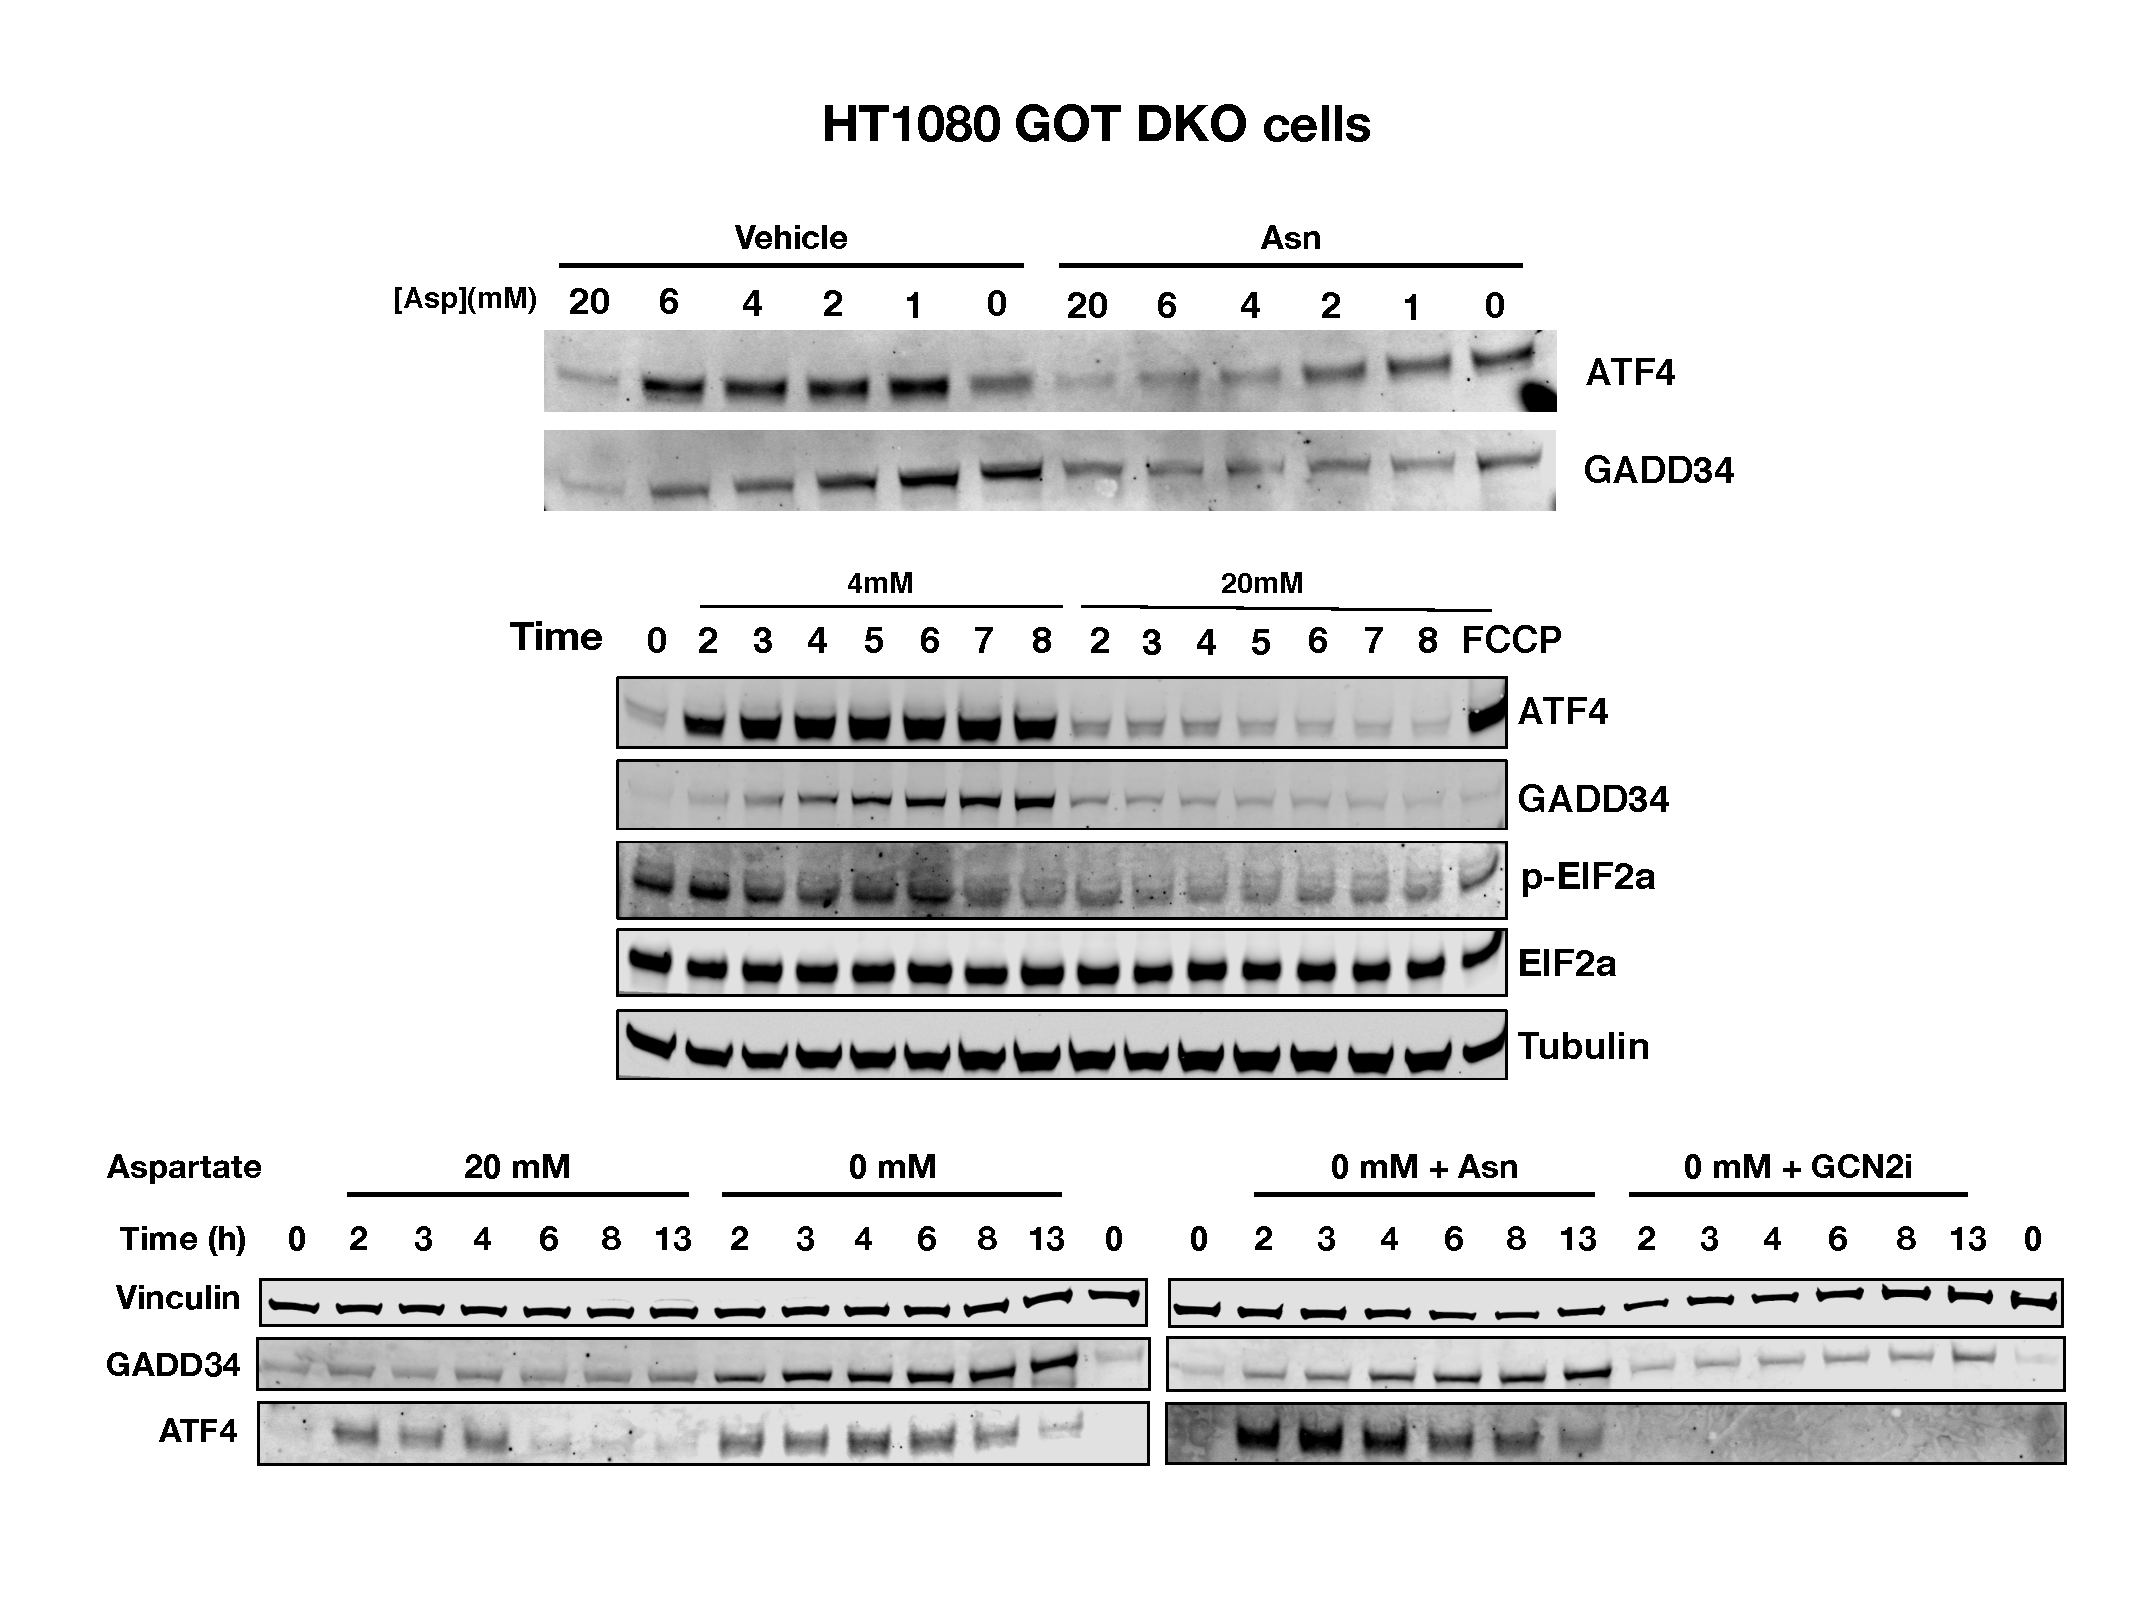
\includegraphics[width=0.99\textwidth]{figures/sapp/ISR/HT1080_DKO_ISR.pdf}
    \caption[Asp depl. induced ISR, HT1080 western]{
    Aspartate depletion in HT1080 GOT DKO cells initiated by media swapping.
    }
    \label{fig:sapp:ISR:HT1080_DKO_ISR}
\end{figure}

\begin{figure}[t]
    \centering
    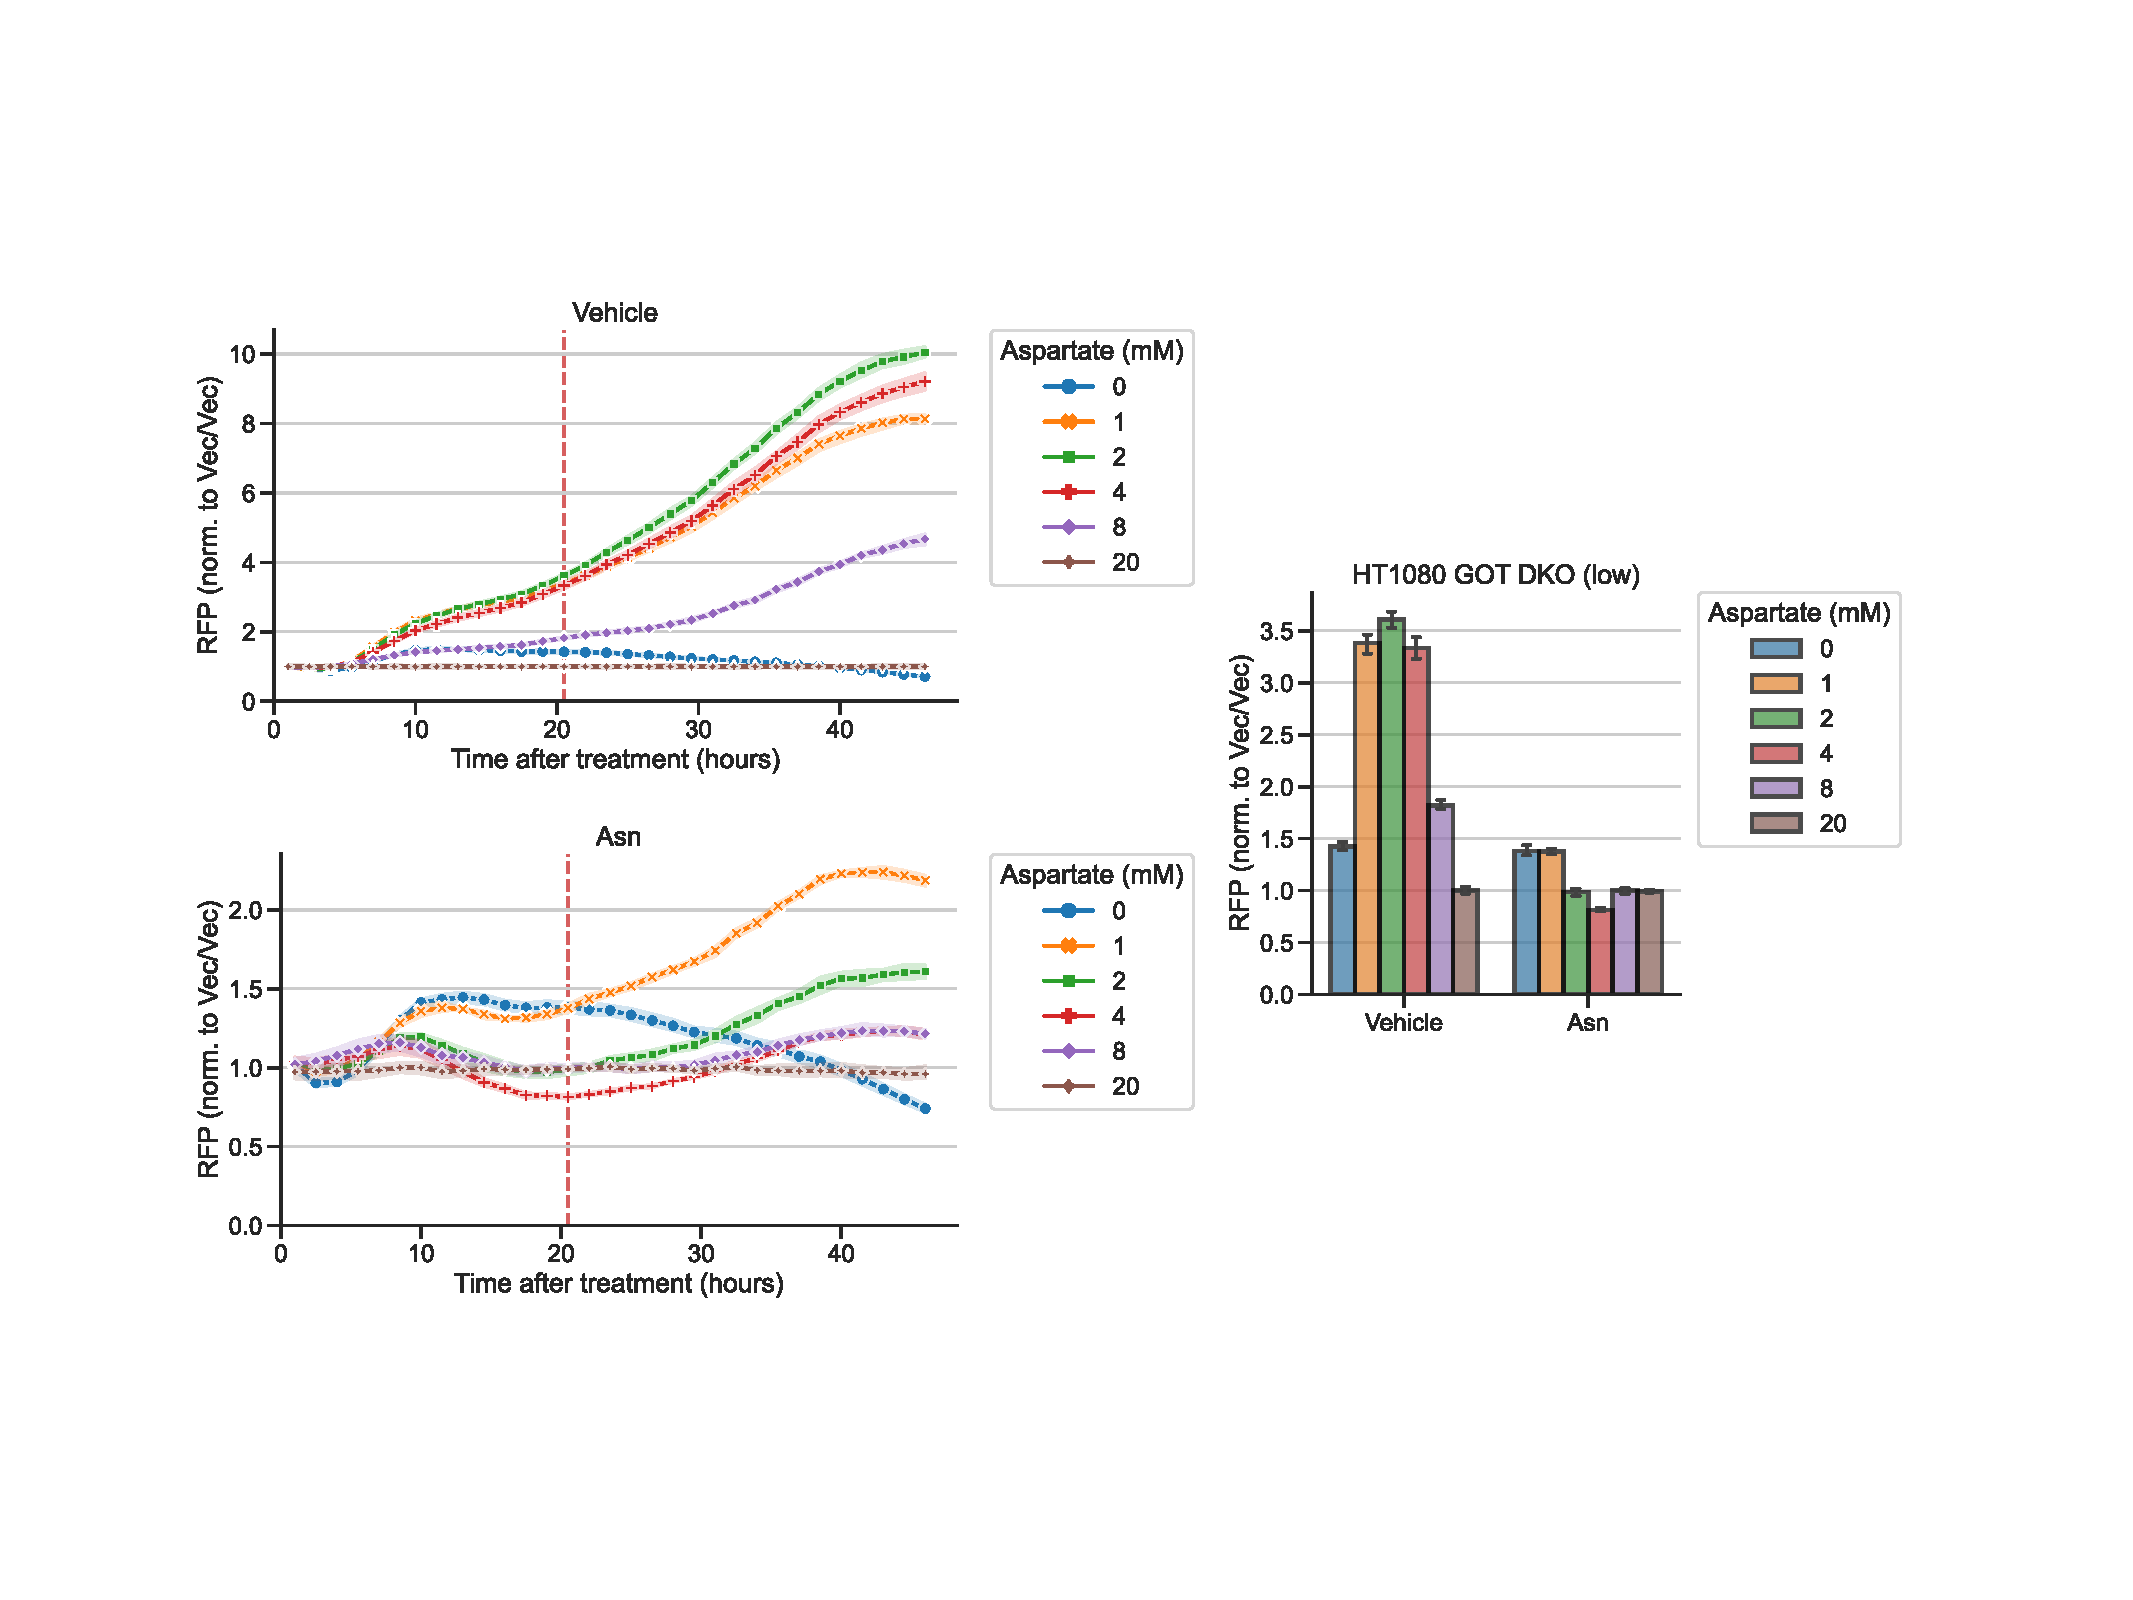
\includegraphics[width=0.98\textwidth]{figures/sapp/ISR/HT1080_DKO_ASPtit_time.pdf}
    \caption[Asp depl. induced ISR, HT1080 ATF4 reporter]{
    ATF4 reporter measurements after aspartate depletion in HT1080 GOT DKO (clone with low reporter at baseline).
    Vec/Vec normalization is normalization to the baseline condition (20 mM Asp, no Asn).
    Vertical red line on curve plot indicates time of measurements extracted for the barplot.
    }
    \label{fig:sapp:ISR:HT1080_DKO_ASPtit_time}
\end{figure}

\begin{figure}[t]
    \centering
    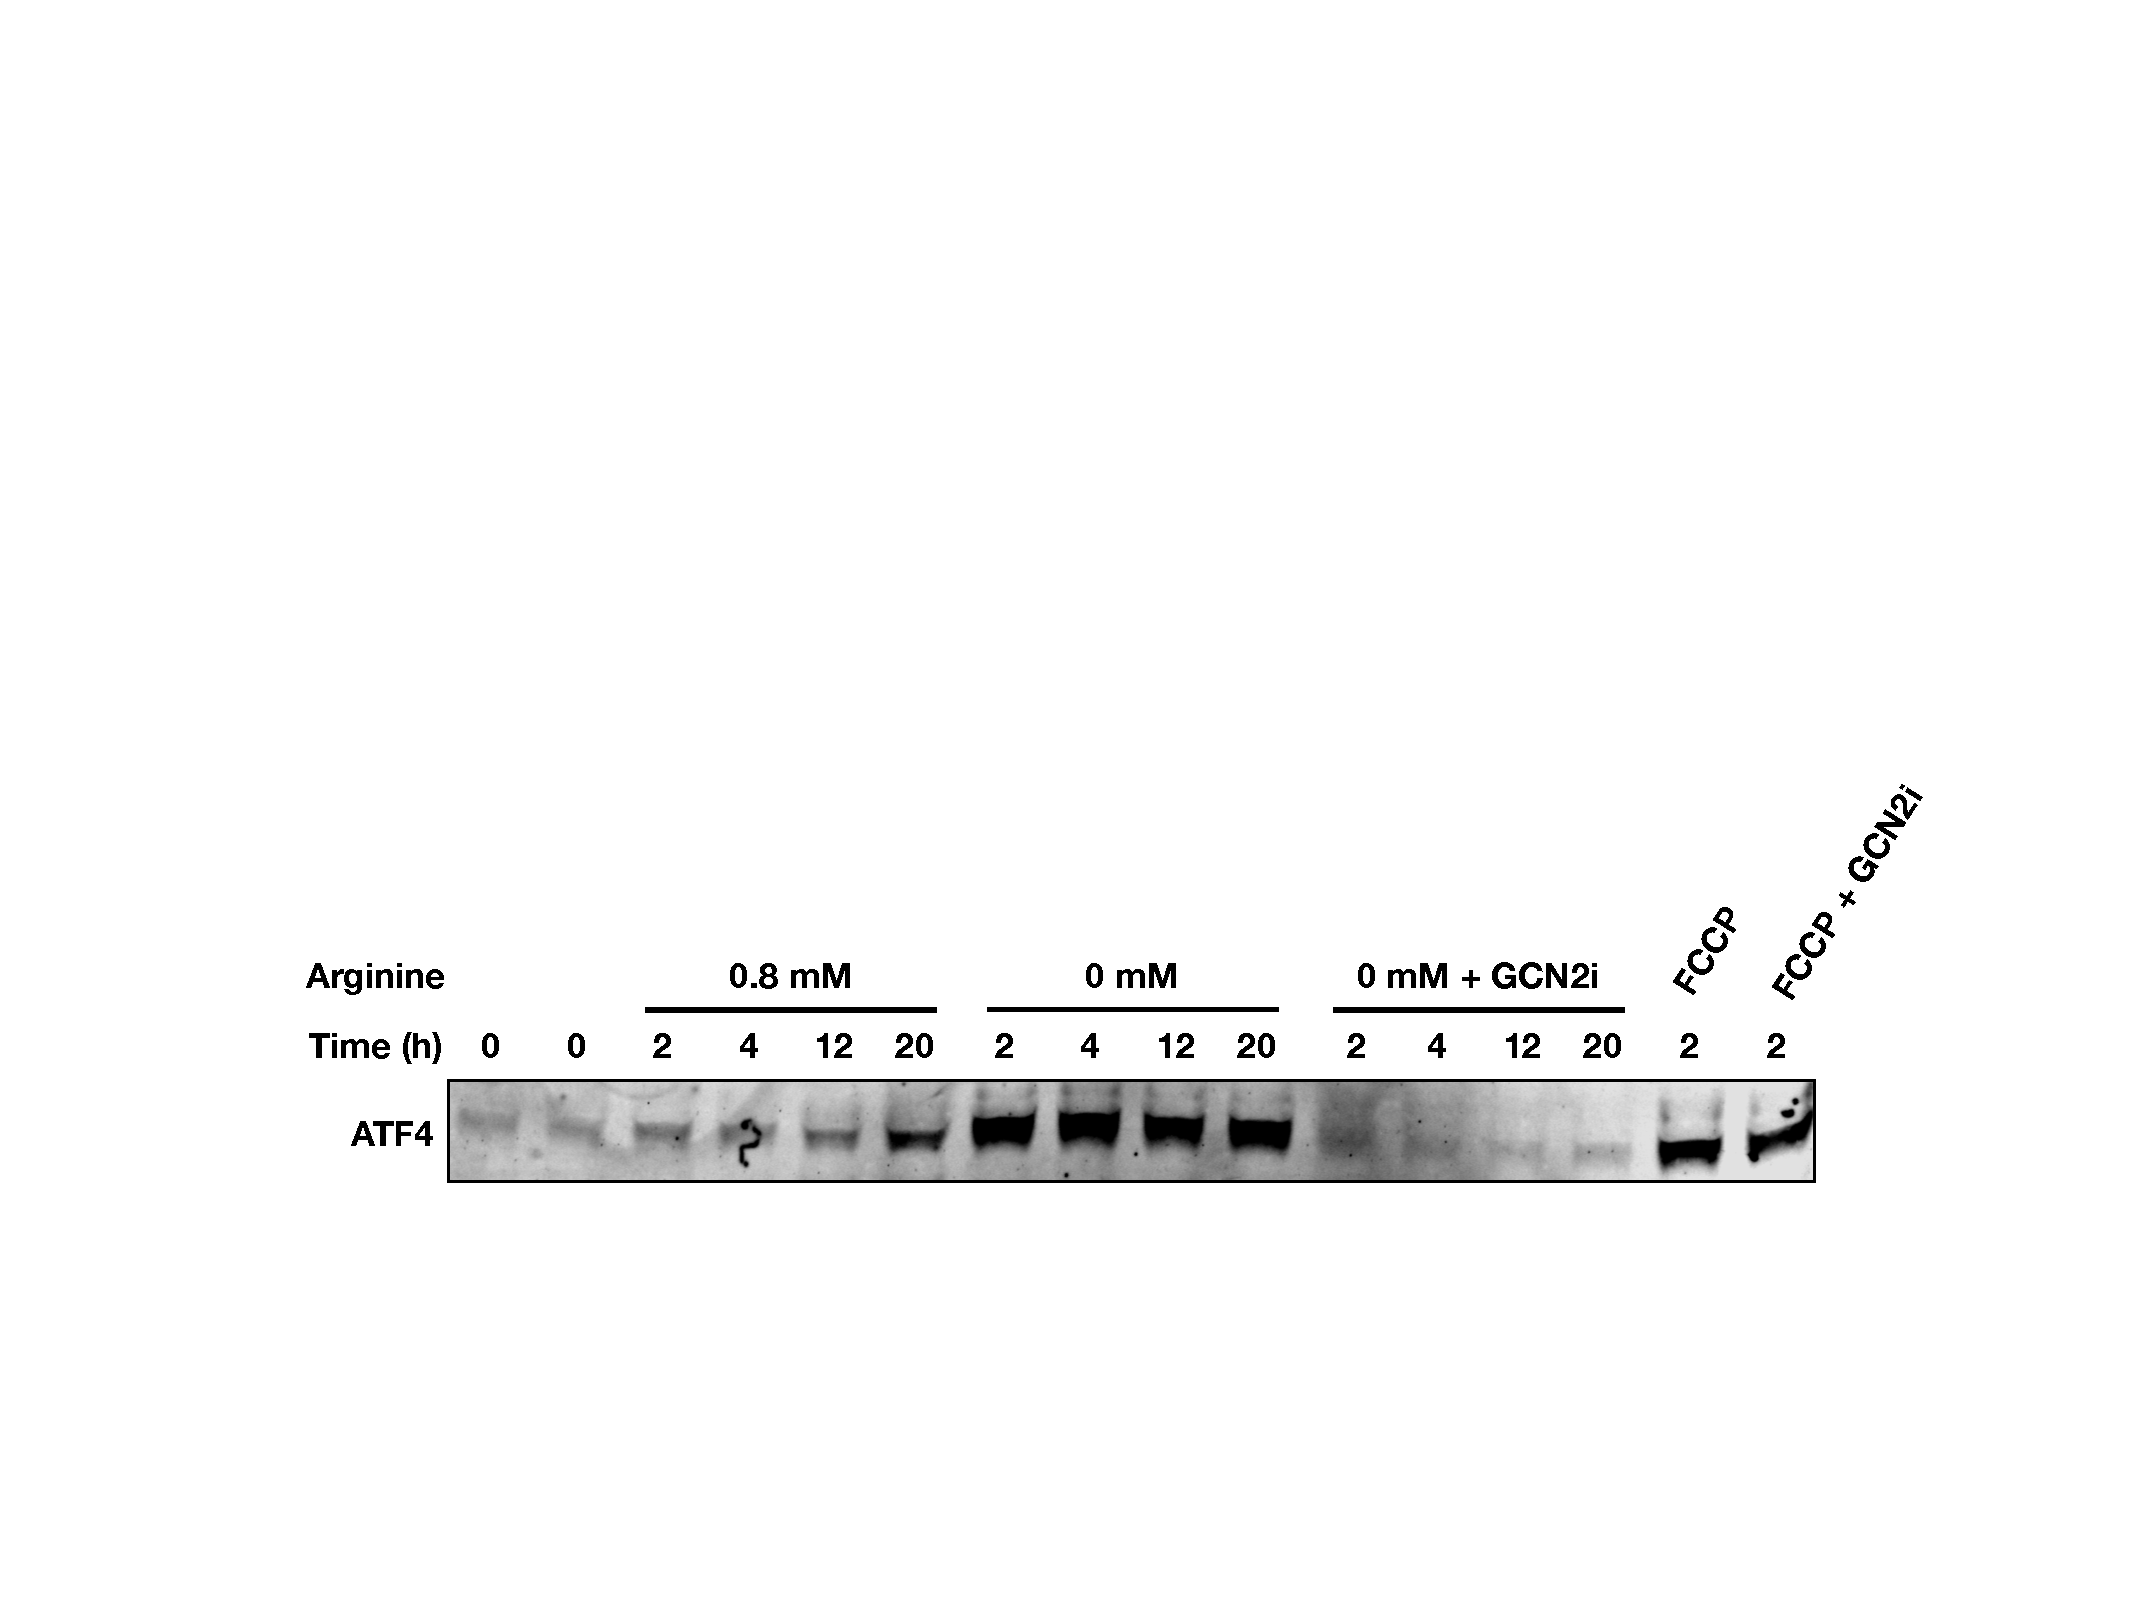
\includegraphics[width=0.60\textwidth]{figures/sapp/ISR/143B_GCN2i_val.pdf}
    \caption[GCN2 inhibitor validation]{
    Validation of activity and specificity of GCN2i in 143B WT cells.
    }
    \label{fig:sapp:ISR:143B_GCN2i_val}
\end{figure}

\begin{figure}[t]
    \centering
    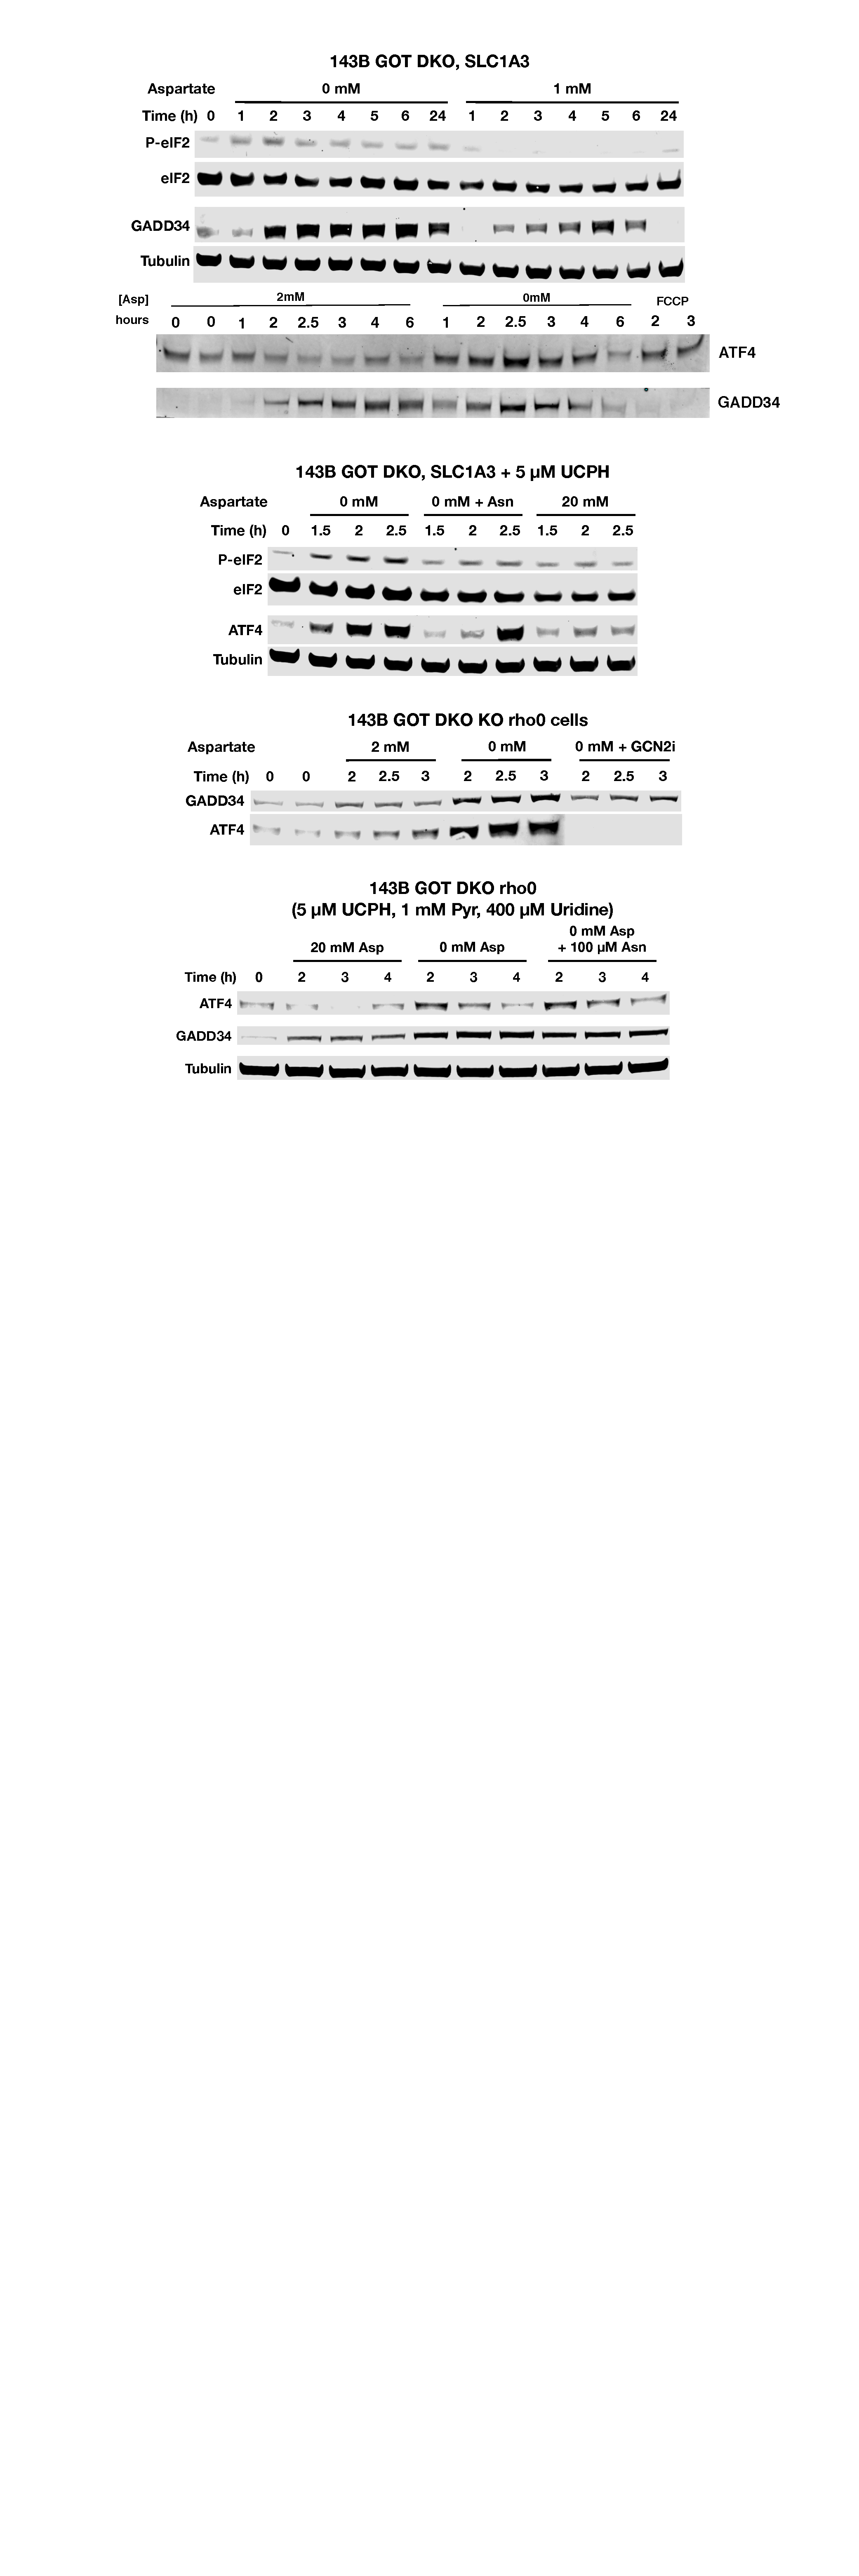
\includegraphics[height=0.85\textheight]{figures/sapp/ISR/143B_DKO_ISR.pdf}
    \caption[Asp depl. induced ISR, 143B western]{
    Aspartate depletion in 143B GOT DKO, SLC1A3 cells initiated by media swapping.
    }
    \label{fig:sapp:ISR:143B_DKO_ISR}
\end{figure}

\begin{figure}[!ht]
     \centering
     \begin{subfigure}[b]{0.35\textwidth}
         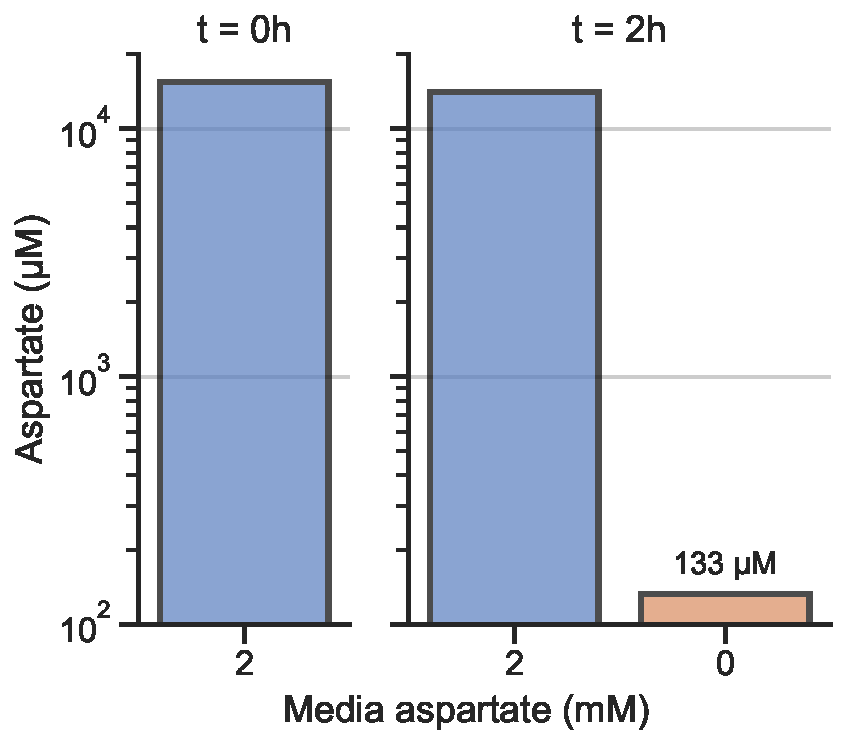
\includegraphics[width=\textwidth]{figures/sapp/ISR/143B_GOT_DKO_ISR_Asp_conc.pdf}
         \caption{Intracellular Asp}
         \label{fig:sapp:ISR:143B_GOT_DKO_ISR_Asp_conc}
     \end{subfigure}
     \hfill
     \begin{subfigure}[b]{0.35\textwidth}
         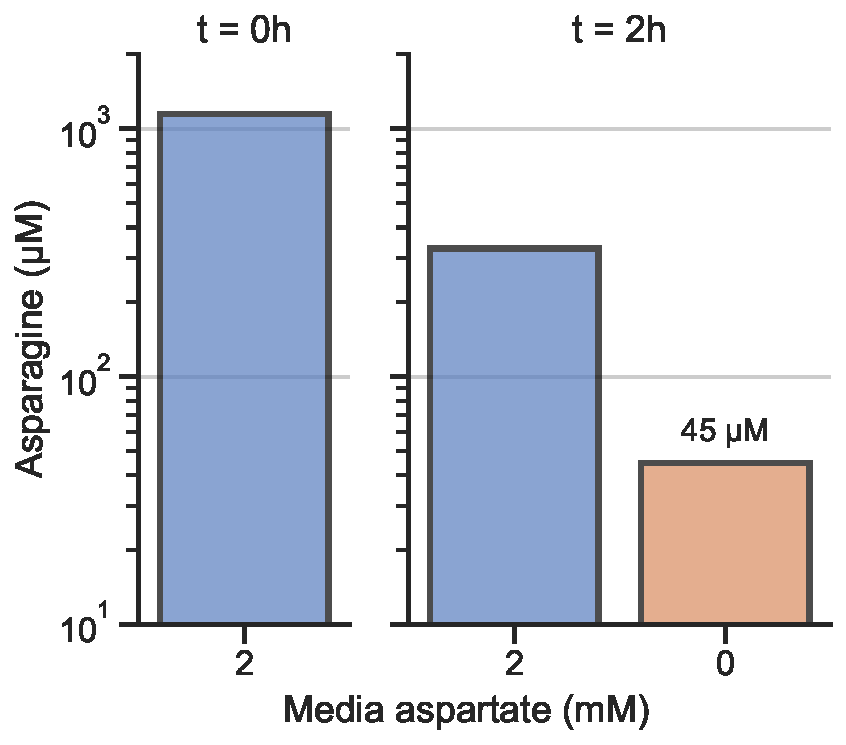
\includegraphics[width=\textwidth]{figures/sapp/ISR/143B_GOT_DKO_ISR_Asn_conc.pdf}
         \caption{Intracellular Asn}
         \label{fig:sapp:ISR:143B_GOT_DKO_ISR_Asn_conc}
     \end{subfigure}
     \hfill
        \caption[Intracellular Asp/Asn at ISR in GOT DKO]{
        Intracellular concentration of aspartate and asparagine before and 2 hours after media switch with/without aspartate for 143B GOT DKO cells, similar to figure \ref{fig:sapp:ISR:143B_DKO_ISR} (second panel from the top).
        }
        \label{fig:sapp:ISR:143B_GOT_DKO_ISR_conc}
\end{figure}





\FloatBarrier
\subsection{OMA1/HRI relation to rotenone/antimycin induced ISR}
According Fessler et al. and Guo et al. \cite{Fessler2020-zk, Guo2020-ia} OMA1/HRI is required for FCCP induced ISR.
Guo et al. also shows OMA1/HRI is required for rotenone/antimycin induced ISR (suppl. of Guo et al.).

We have knockout cells (parental HT1080 ATF reporter low clone) of OMA1 and HRI.
These appear to ablate rotenone/antimycin induced ISR but strangely not FCCP induced ISR.
This could be due to pleiotropic effect of FCCP e.g. its is also depolarizing the plasma membrane and the lysosomal membrane.

\begin{figure}[!ht]
     \centering
     \begin{subfigure}[b]{0.49\textwidth}
         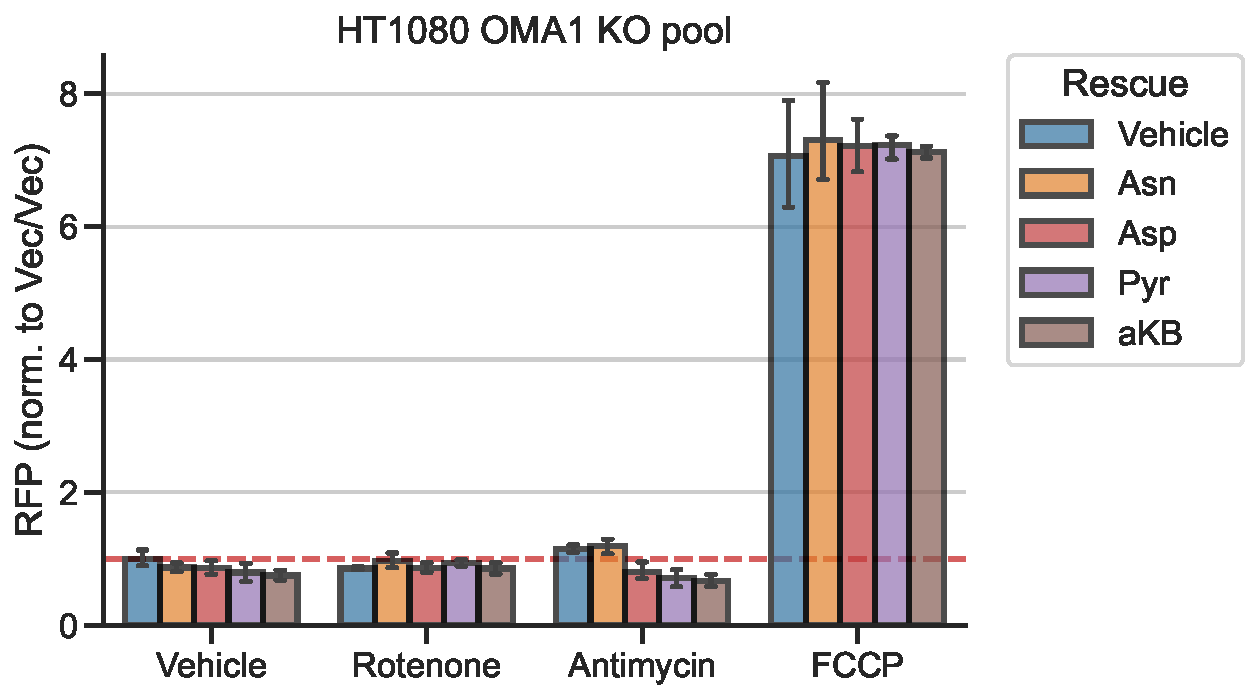
\includegraphics[width=\textwidth]{figures/sapp/ISR/ATF4rep_OMA1pool.pdf}
         \caption{OMA1 KO pool}
         \label{fig:sapp:ISR:ATF4rep_OMA1pool}
     \end{subfigure}
     \hfill
     \begin{subfigure}[b]{0.49\textwidth}
         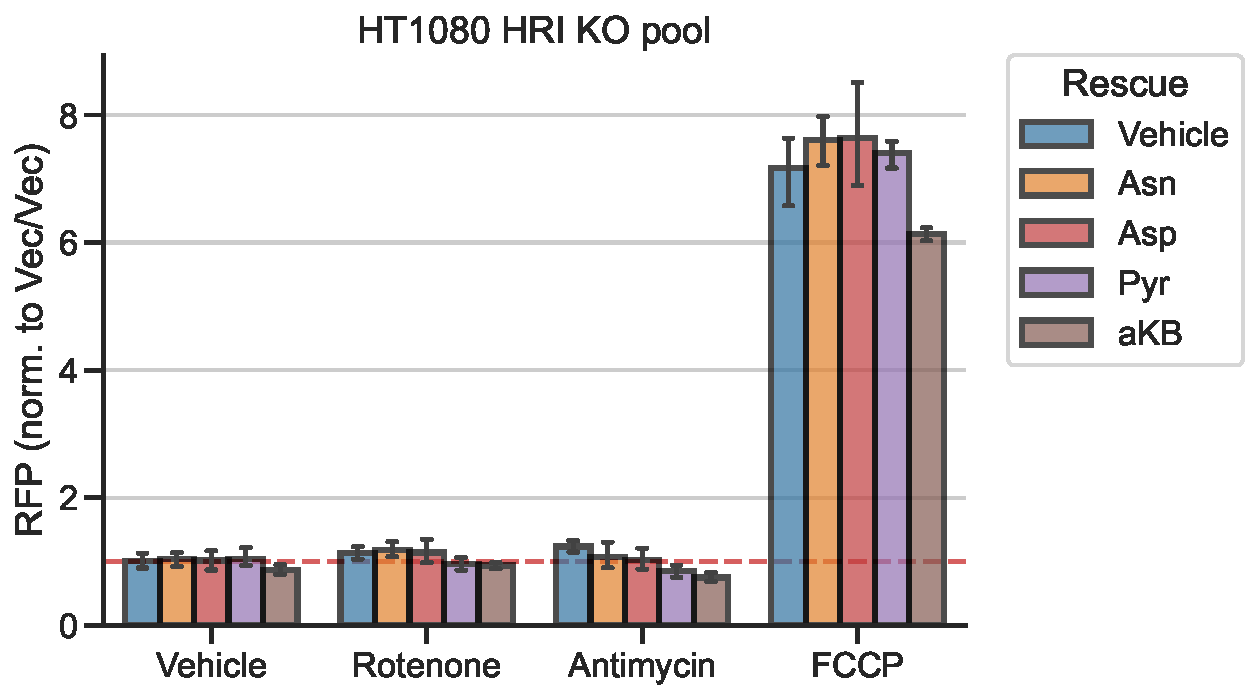
\includegraphics[width=\textwidth]{figures/sapp/ISR/ATF4rep_HRIpool.pdf}
         \caption{HRI KO pool}
         \label{fig:sapp:ISR:ATF4rep_HRIpool}
     \end{subfigure}
     \hfill
        \caption[ATF4 post mito inhib. OMA1/HRI KO, reporter]{
        ATF4 reporter assay measured 21 h after drug treatment with vehicle, rotenone (100 nM) or antimycin (1 µM) spiked-in as 10x.
        }
        \label{fig:sapp:ISR:ATF4rep_OMA1_HRIpool}
\end{figure}

\begin{figure}[t]
    \centering
    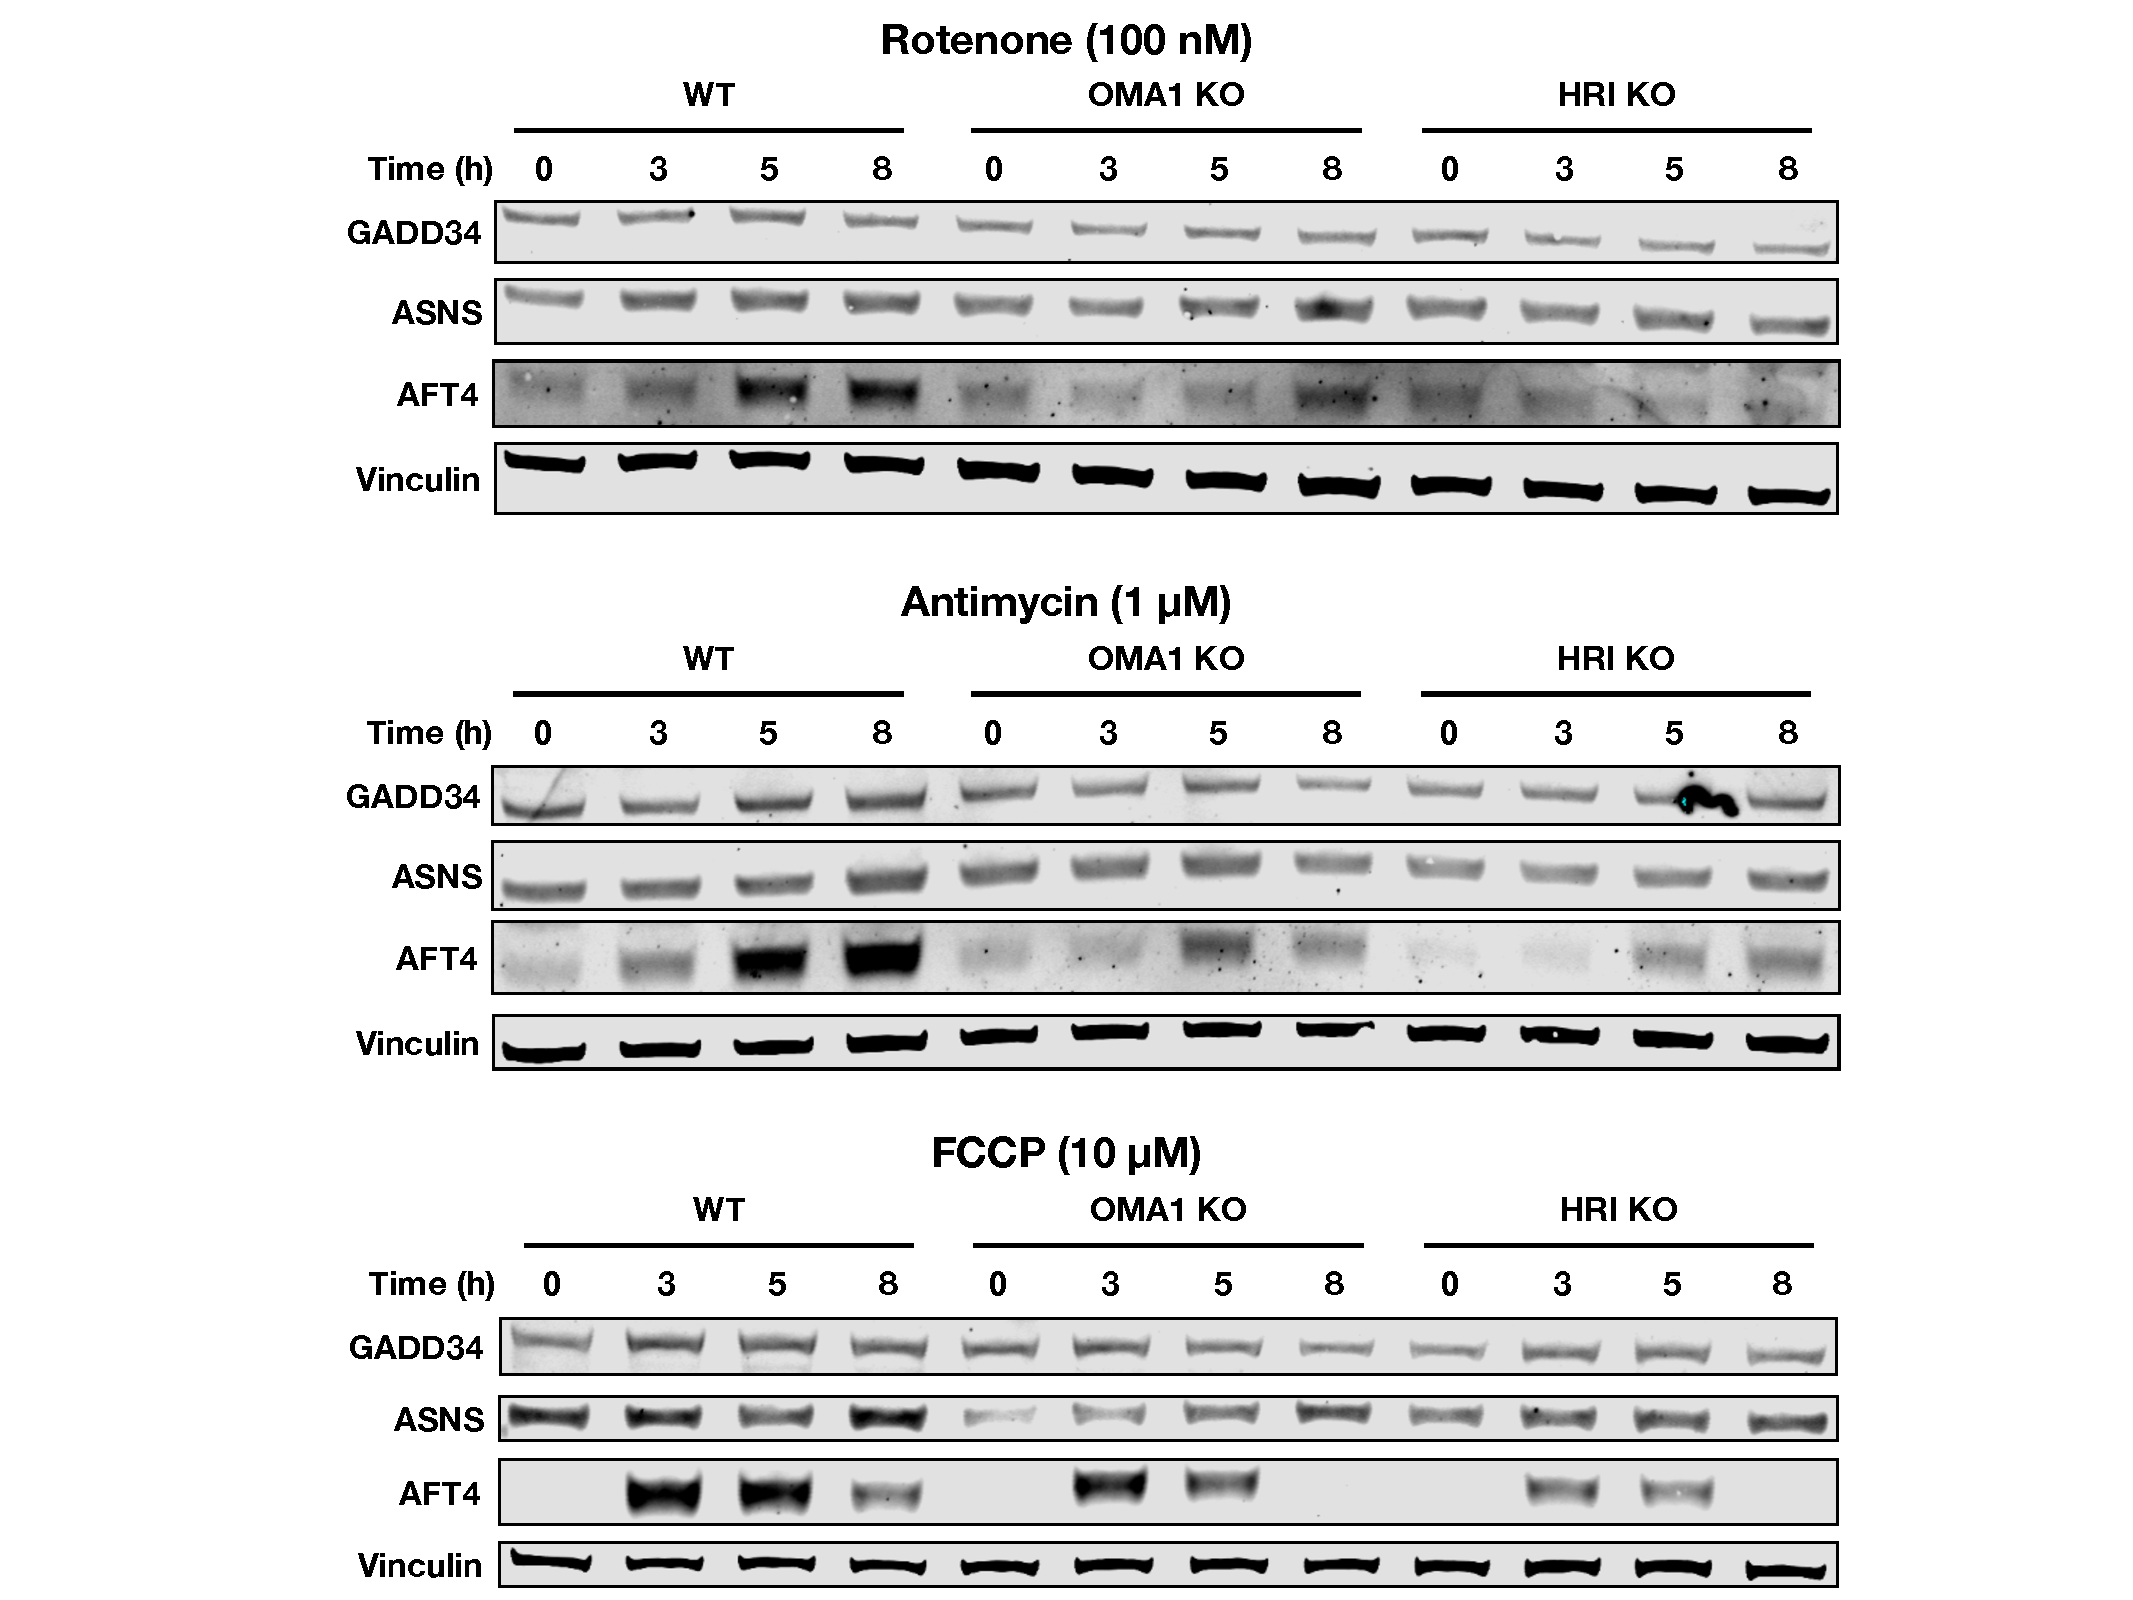
\includegraphics[width=0.65\textwidth]{figures/sapp/ISR/ATF4wes_OMA1_HRIpool.pdf}
    \caption[ATF4 post mito inhib. OMA1/HRI KO, western]{
    Same pooled knockout cells and handling as in figure \ref{fig:sapp:ISR:ATF4rep_OMA1_HRIpool}.
    Drugs spiked-in as 10x.
    }
    \label{fig:sapp:ISR:ATF4wes_OMA1_HRIpool}
\end{figure}






\FloatBarrier
\subsection{OMA1/HRI relation to asp depletion induced ISR}
OMA1 KO appears on western blot to ablate ATF4 upregulation in response to aspartate depletion; however, HRI does not.
Another experiment, exclusively with OMA1, shows that it is not required for ATF4 upregulation after aspartate depletion, on the other hand GCN2 appears to be required.

If OMA1/HRI is involved with aspartate depletion induced ISR it could be through altering the mitochondrial membrane potential.
Aspartate depletion would prevent the malate-aspartate from shuttling electrons into the inner mitochondria, a process which is, presumably, still active in GOT DKO cells.
Aspartate is exported out of the mitochondria using the membrane potential i.e. one aspartate out for one glutamate and a proton in.
Thus, depleting cytoplasmic aspartate might alter the membrane potential in unpredictable ways and indeed there appears to be a small increase in mitochondrial membrane potential in HT1080 GOT DKO cells as aspartate is progressively depleted from the media (figure \ref{fig:sapp:ISR:HT1080_GOT_DKO_TMRE}).

\begin{figure}
    \centering
    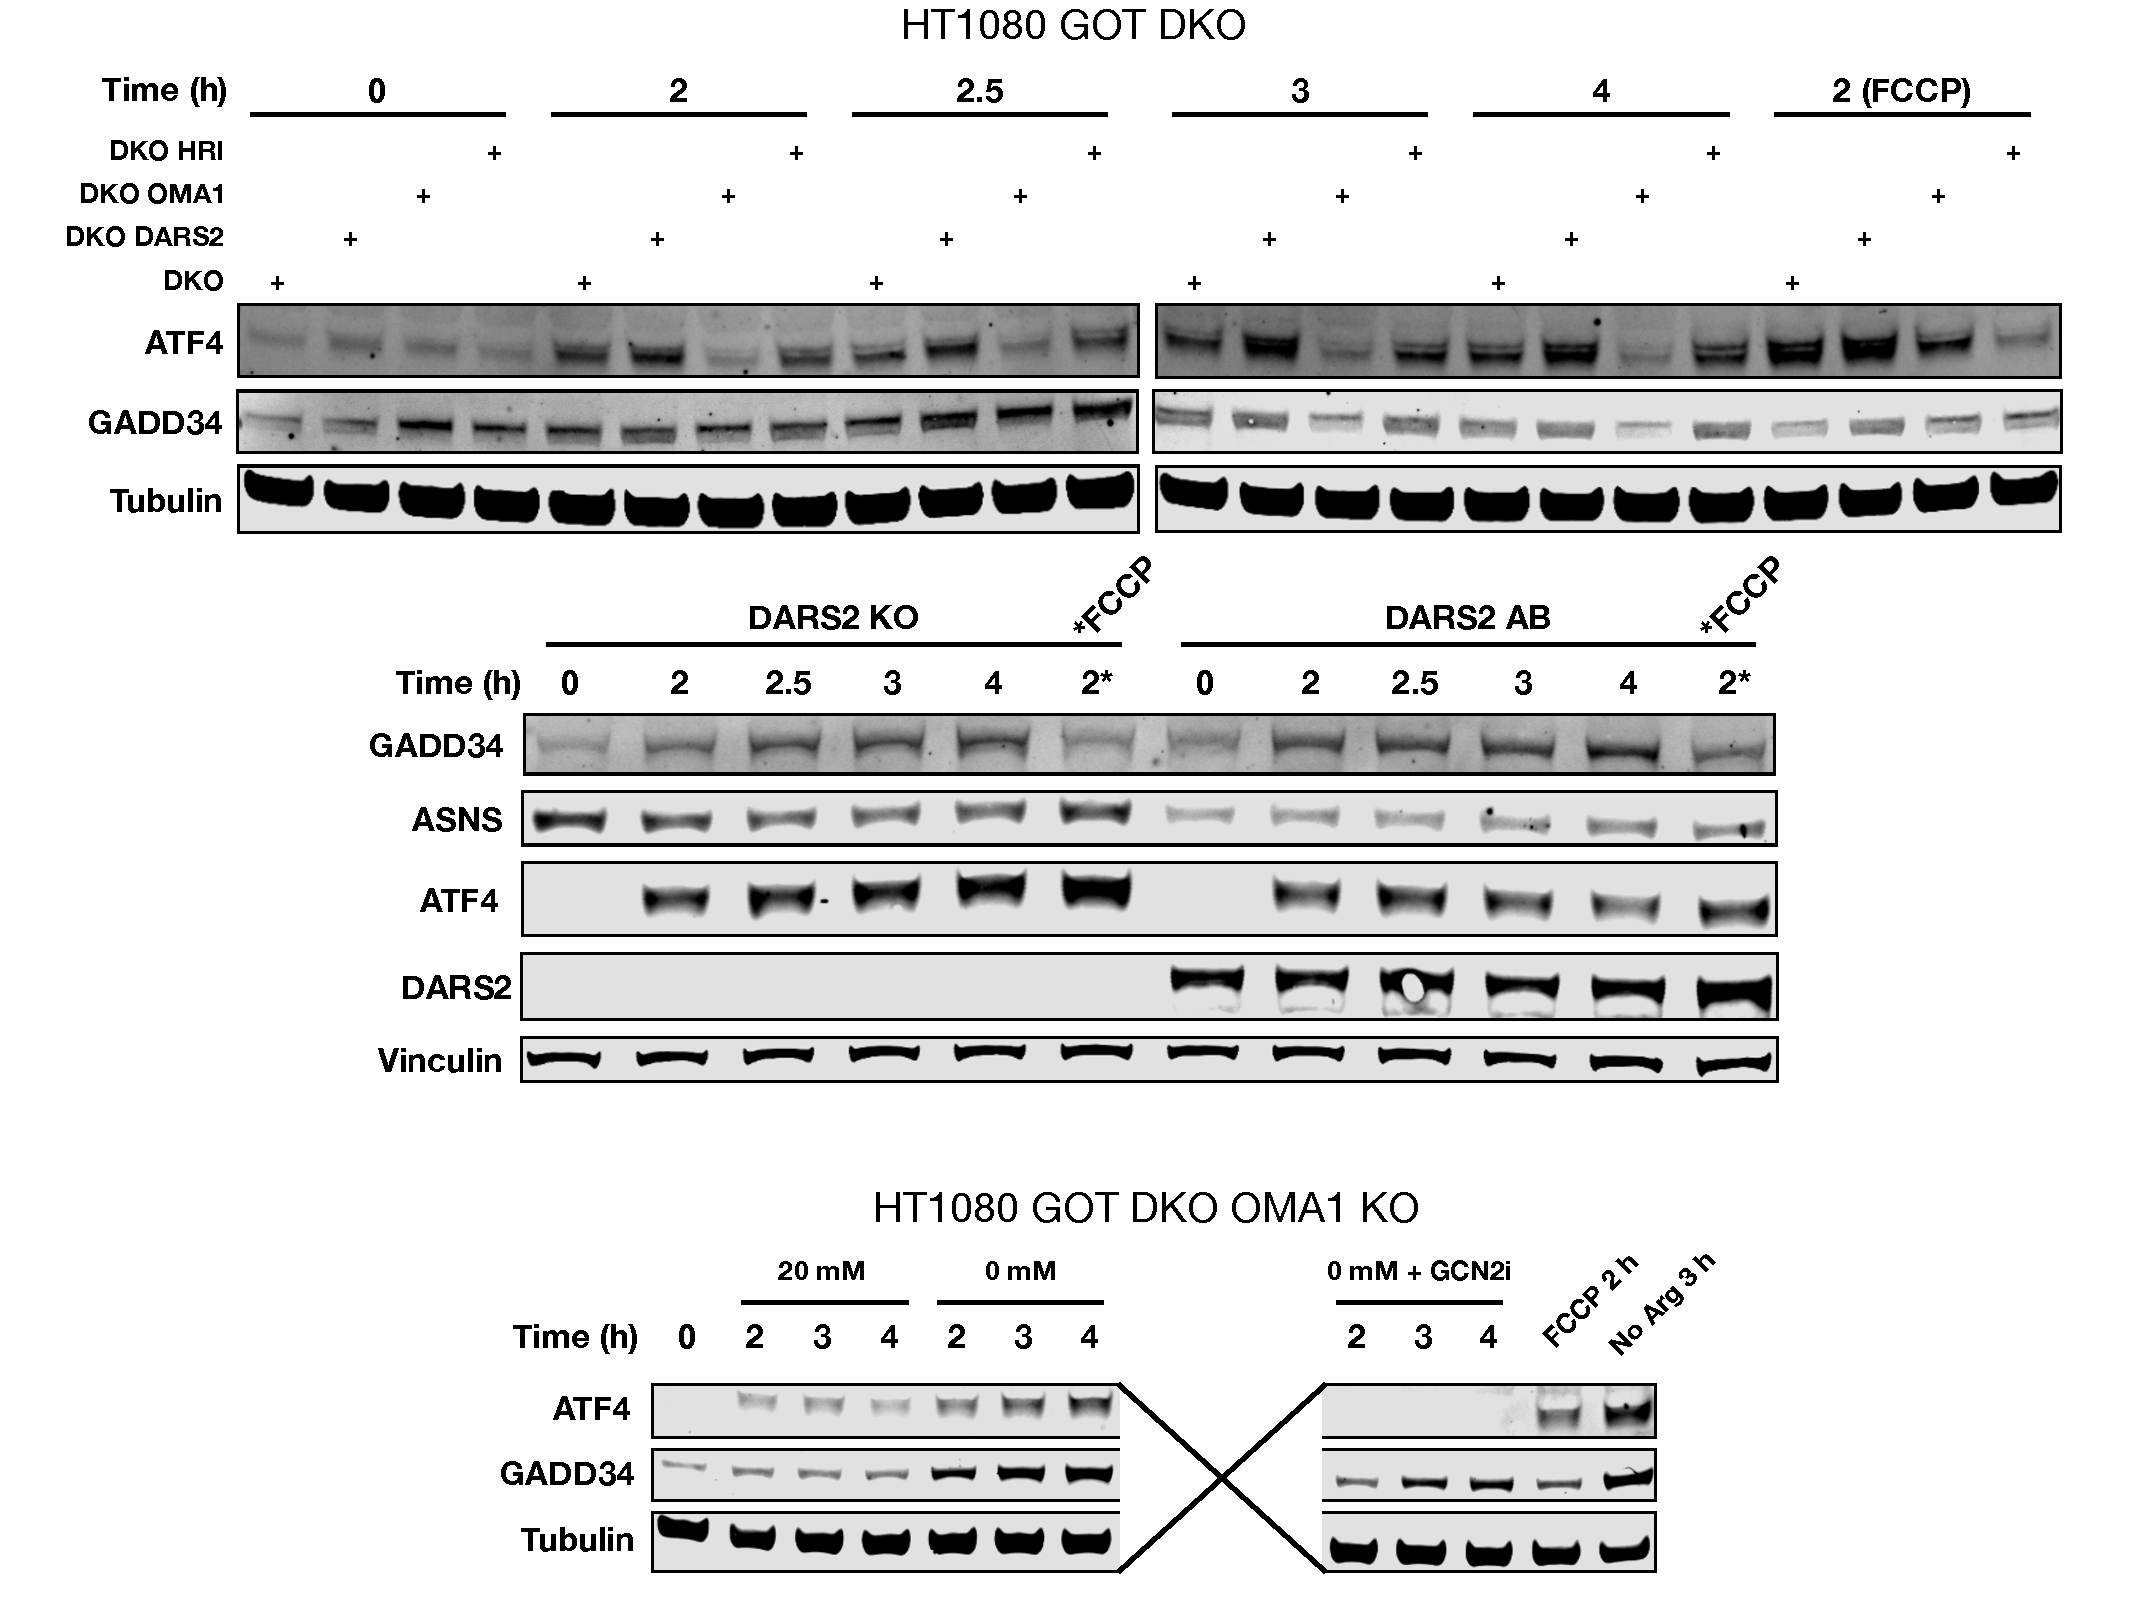
\includegraphics[width=0.95\textwidth]{figures/sapp/ISR/HT1080_DKO_KO_ISR.pdf}
    \caption[ATF4 post Asp depl. OMA1/HRI KO, western]{
    Effect of OMA1, HRI or DARS2 KO on aspartate depletion induced ISR.
    Single cell clones validated for OMA1 and DARS2, only functionally validated for HRI, see figure \ref{fig:sapp:ISR:OMA1_HRI_DARS2_val}.
    Aspartate depletion initiated by switching to media with no asp at time zero.
    Irrelevant well spliced out.
    }
    \label{fig:sapp:ISR:HT1080_DKO_KO_ISR}
\end{figure}

\begin{figure}
     \centering
     \begin{subfigure}[b]{0.49\textwidth}
         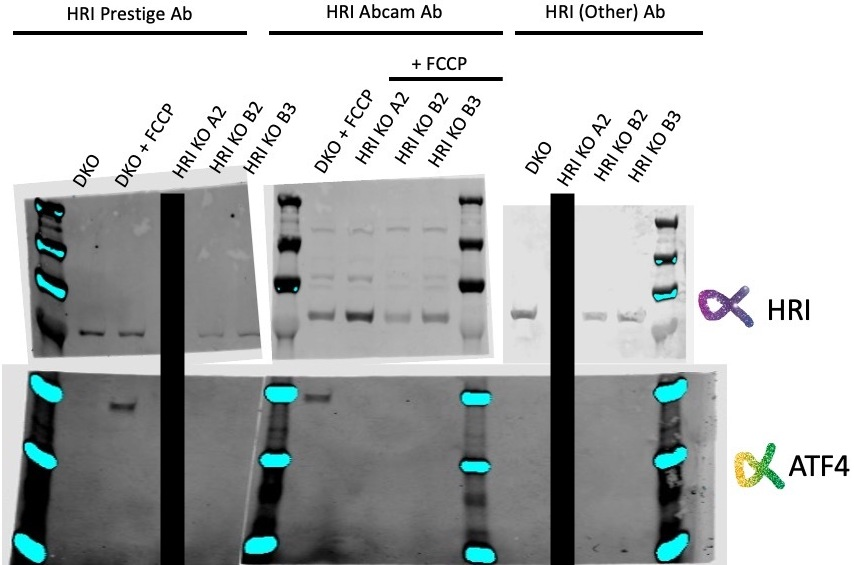
\includegraphics[width=\textwidth]{figures/sapp/ISR/HT1080_GOT_DKO_HRI_KO.jpeg}
         \caption{HT1080 GOT DKO, HRI KO}
         \label{fig:sapp:ISR:HT1080_GOT_DKO_HRI_KO}
     \end{subfigure}
     \hfill
     \begin{subfigure}[b]{0.49\textwidth}
         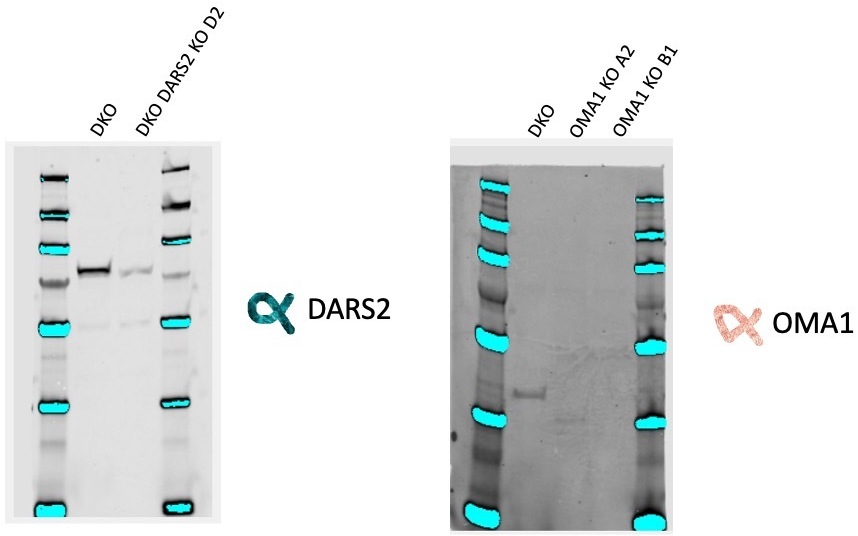
\includegraphics[width=\textwidth]{figures/sapp/ISR/HT1080_GOT_DKO_OMA1_DARS2_KO.jpeg}
         \caption{HT1080 GOT DKO, OMA1/DARS2 KO}
         \label{fig:sapp:ISR:HT1080_GOT_DKO_OMA1_DARS2_KO}
     \end{subfigure}
     \hfill
        \caption[HT1080 GOT DKO, OMA1/HRI/DARS2 KO validation]{
        Western blot validations of OMA1, HRI and DARS2 knockouts.
        Image art credit: Ian Engstrom.
        }
        \label{fig:sapp:ISR:OMA1_HRI_DARS2_val}
\end{figure}

\begin{figure}[!ht]
     \centering
     \begin{subfigure}[b]{0.65\textwidth}
         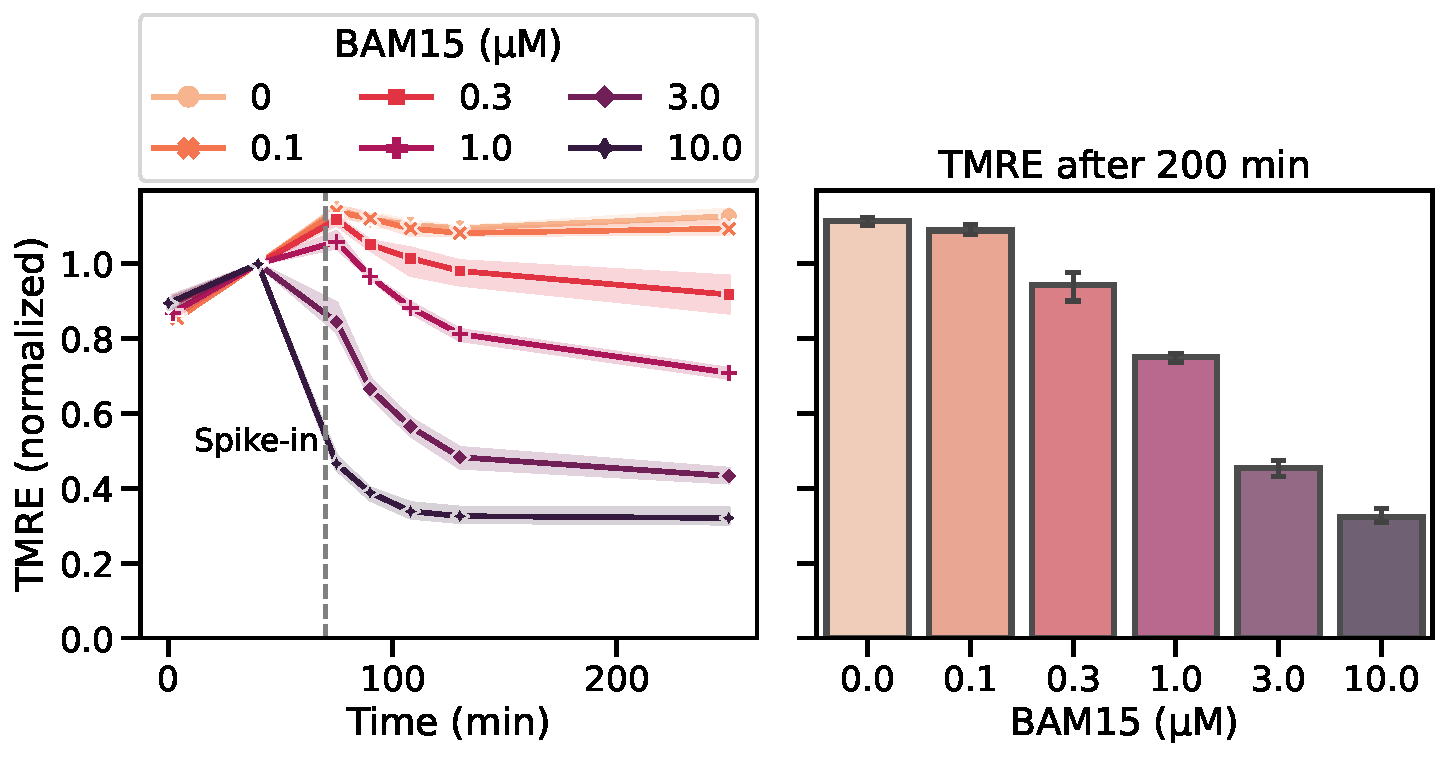
\includegraphics[width=\textwidth]{figures/sapp/ISR/HT1080_GOT_DKO_TMRA_BAM15tit.pdf}
         \caption{BAM15, mito membrane potential}
         \label{fig:sapp:ISR:HT1080_GOT_DKO_TMRA_BAM15tit}
     \end{subfigure}
     \hfill
     \begin{subfigure}[b]{0.8\textwidth}
         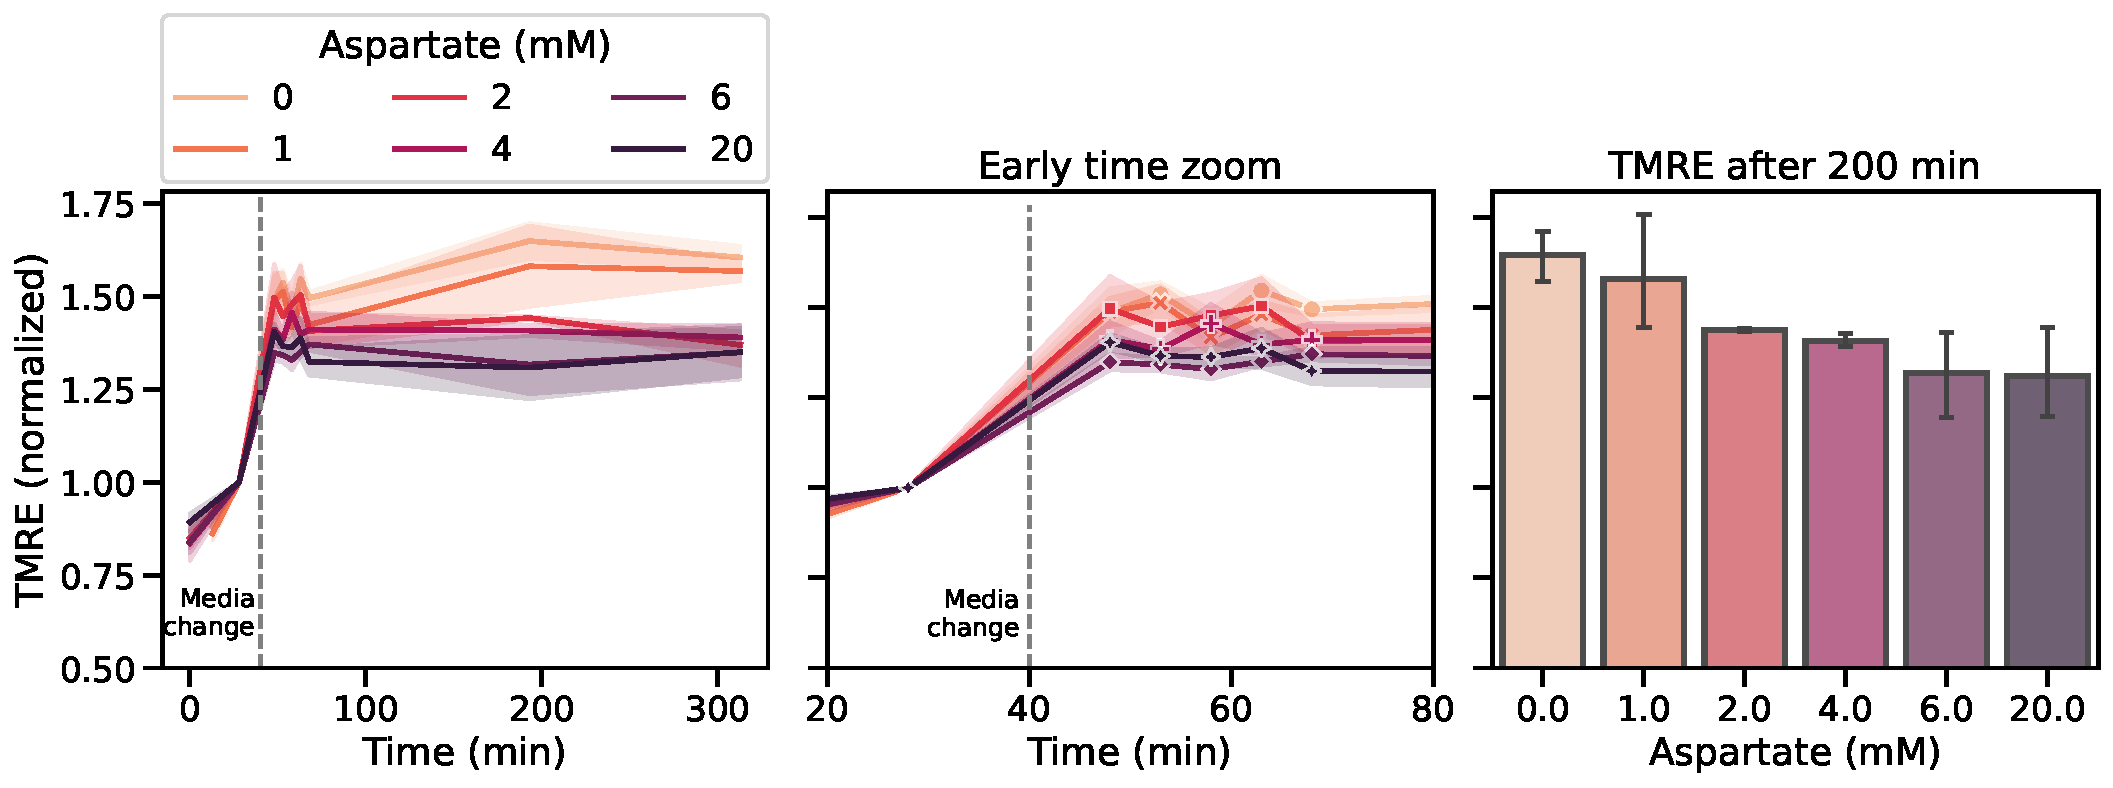
\includegraphics[width=\textwidth]{figures/sapp/ISR/HT1080_GOT_DKO_TMRA_ASPtit.pdf}
         \caption{Asp depletion, mito membrane potential}
         \label{fig:sapp:ISR:HT1080_GOT_DKO_TMRA_ASPtit}
     \end{subfigure}
     \hfill
        \caption[Mito membrane potential in GOT DKO]{
        Mitochondrial membrane potential increases slightly during aspartate depletion in HT1080 GOT DKO.
        Measured on an Incucyte using the TMRE dye.
        }
        \label{fig:sapp:ISR:HT1080_GOT_DKO_TMRE}
\end{figure}











\FloatBarrier
\subsection{ASNS over-expression to ablate rotenone/antimycin induced ISR}
If asparagine depletion is the main reason for rotenone/antimycin induced ISR maybe over-expression of ASNS would mitigate it?
Using the HT1080 ATF4 reporter cells (low baseline clone) ASNS and eGFP (control) was over-expressed using lentiviral infection.
The polyclonal population that grew out after selection was tested for ATF4 upregulation using reporter assay and western blot.
Generally, ASNS over-expression diminish ATF4 upregulation, but strangely, in this background, adding additional asparagine increase ATF4.

\begin{figure}
     \centering
     \begin{subfigure}[b]{0.49\textwidth}
         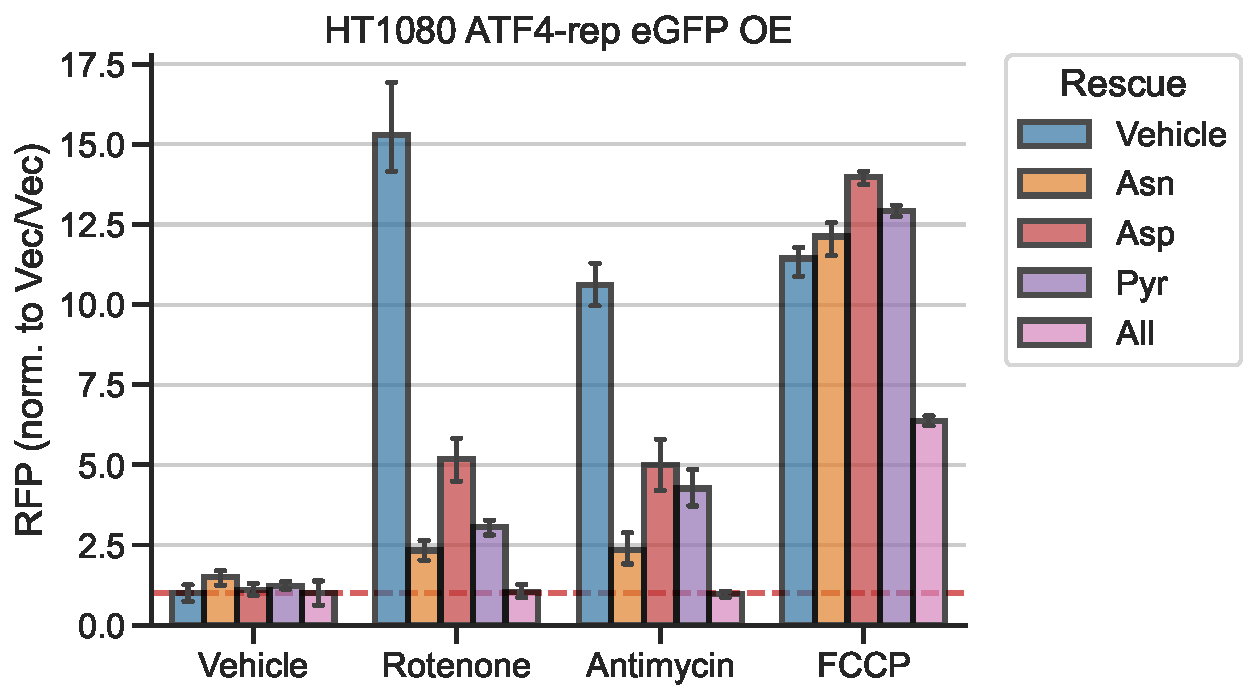
\includegraphics[width=\textwidth]{figures/sapp/ISR/HT1080_ATF4rep_eGFP_OE.pdf}
         \caption{ATF4 reporter, eGFP polyclonal}
         \label{fig:sapp:ISR:HT1080_ATF4rep_eGFP_OE}
     \end{subfigure}
     \hfill
     \begin{subfigure}[b]{0.49\textwidth}
         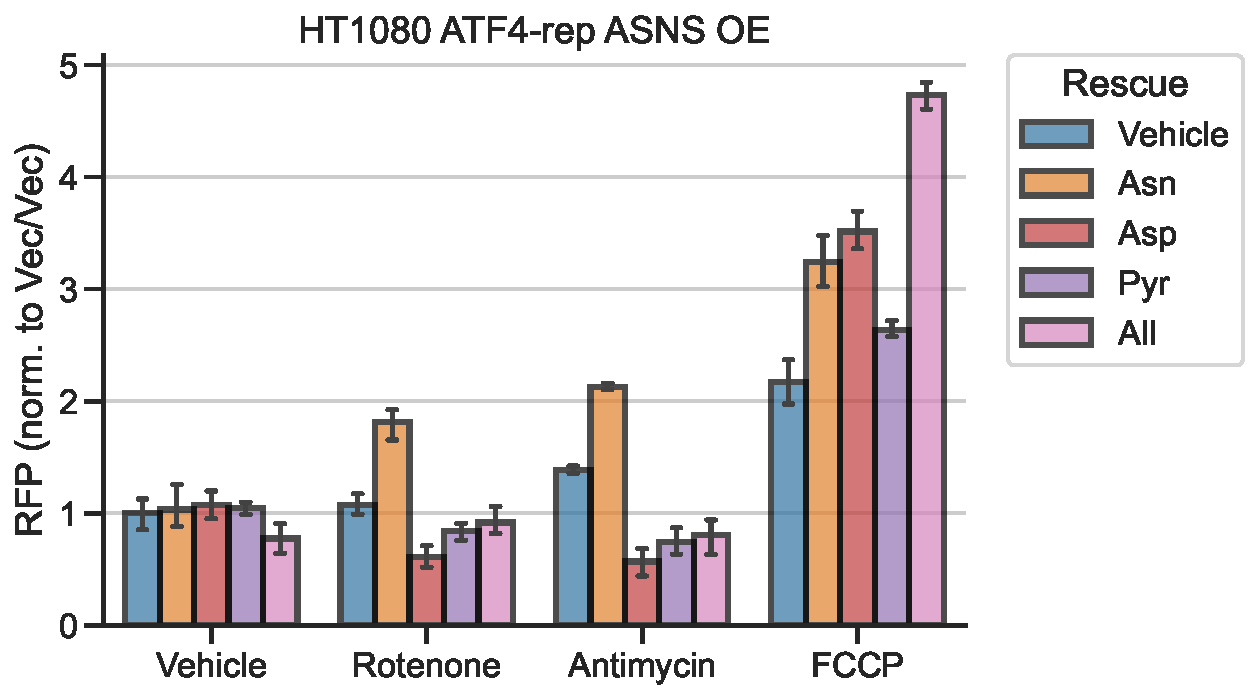
\includegraphics[width=\textwidth]{figures/sapp/ISR/HT1080_ATF4rep_ASNS_OE.pdf}
         \caption{ATF4 reporter, ASNS polyclonal}
         \label{fig:sapp:ISR:HT1080_ATF4rep_ASNS_OE}
     \end{subfigure}
     \hfill
     \begin{subfigure}[b]{0.6\textwidth}
         \centering
         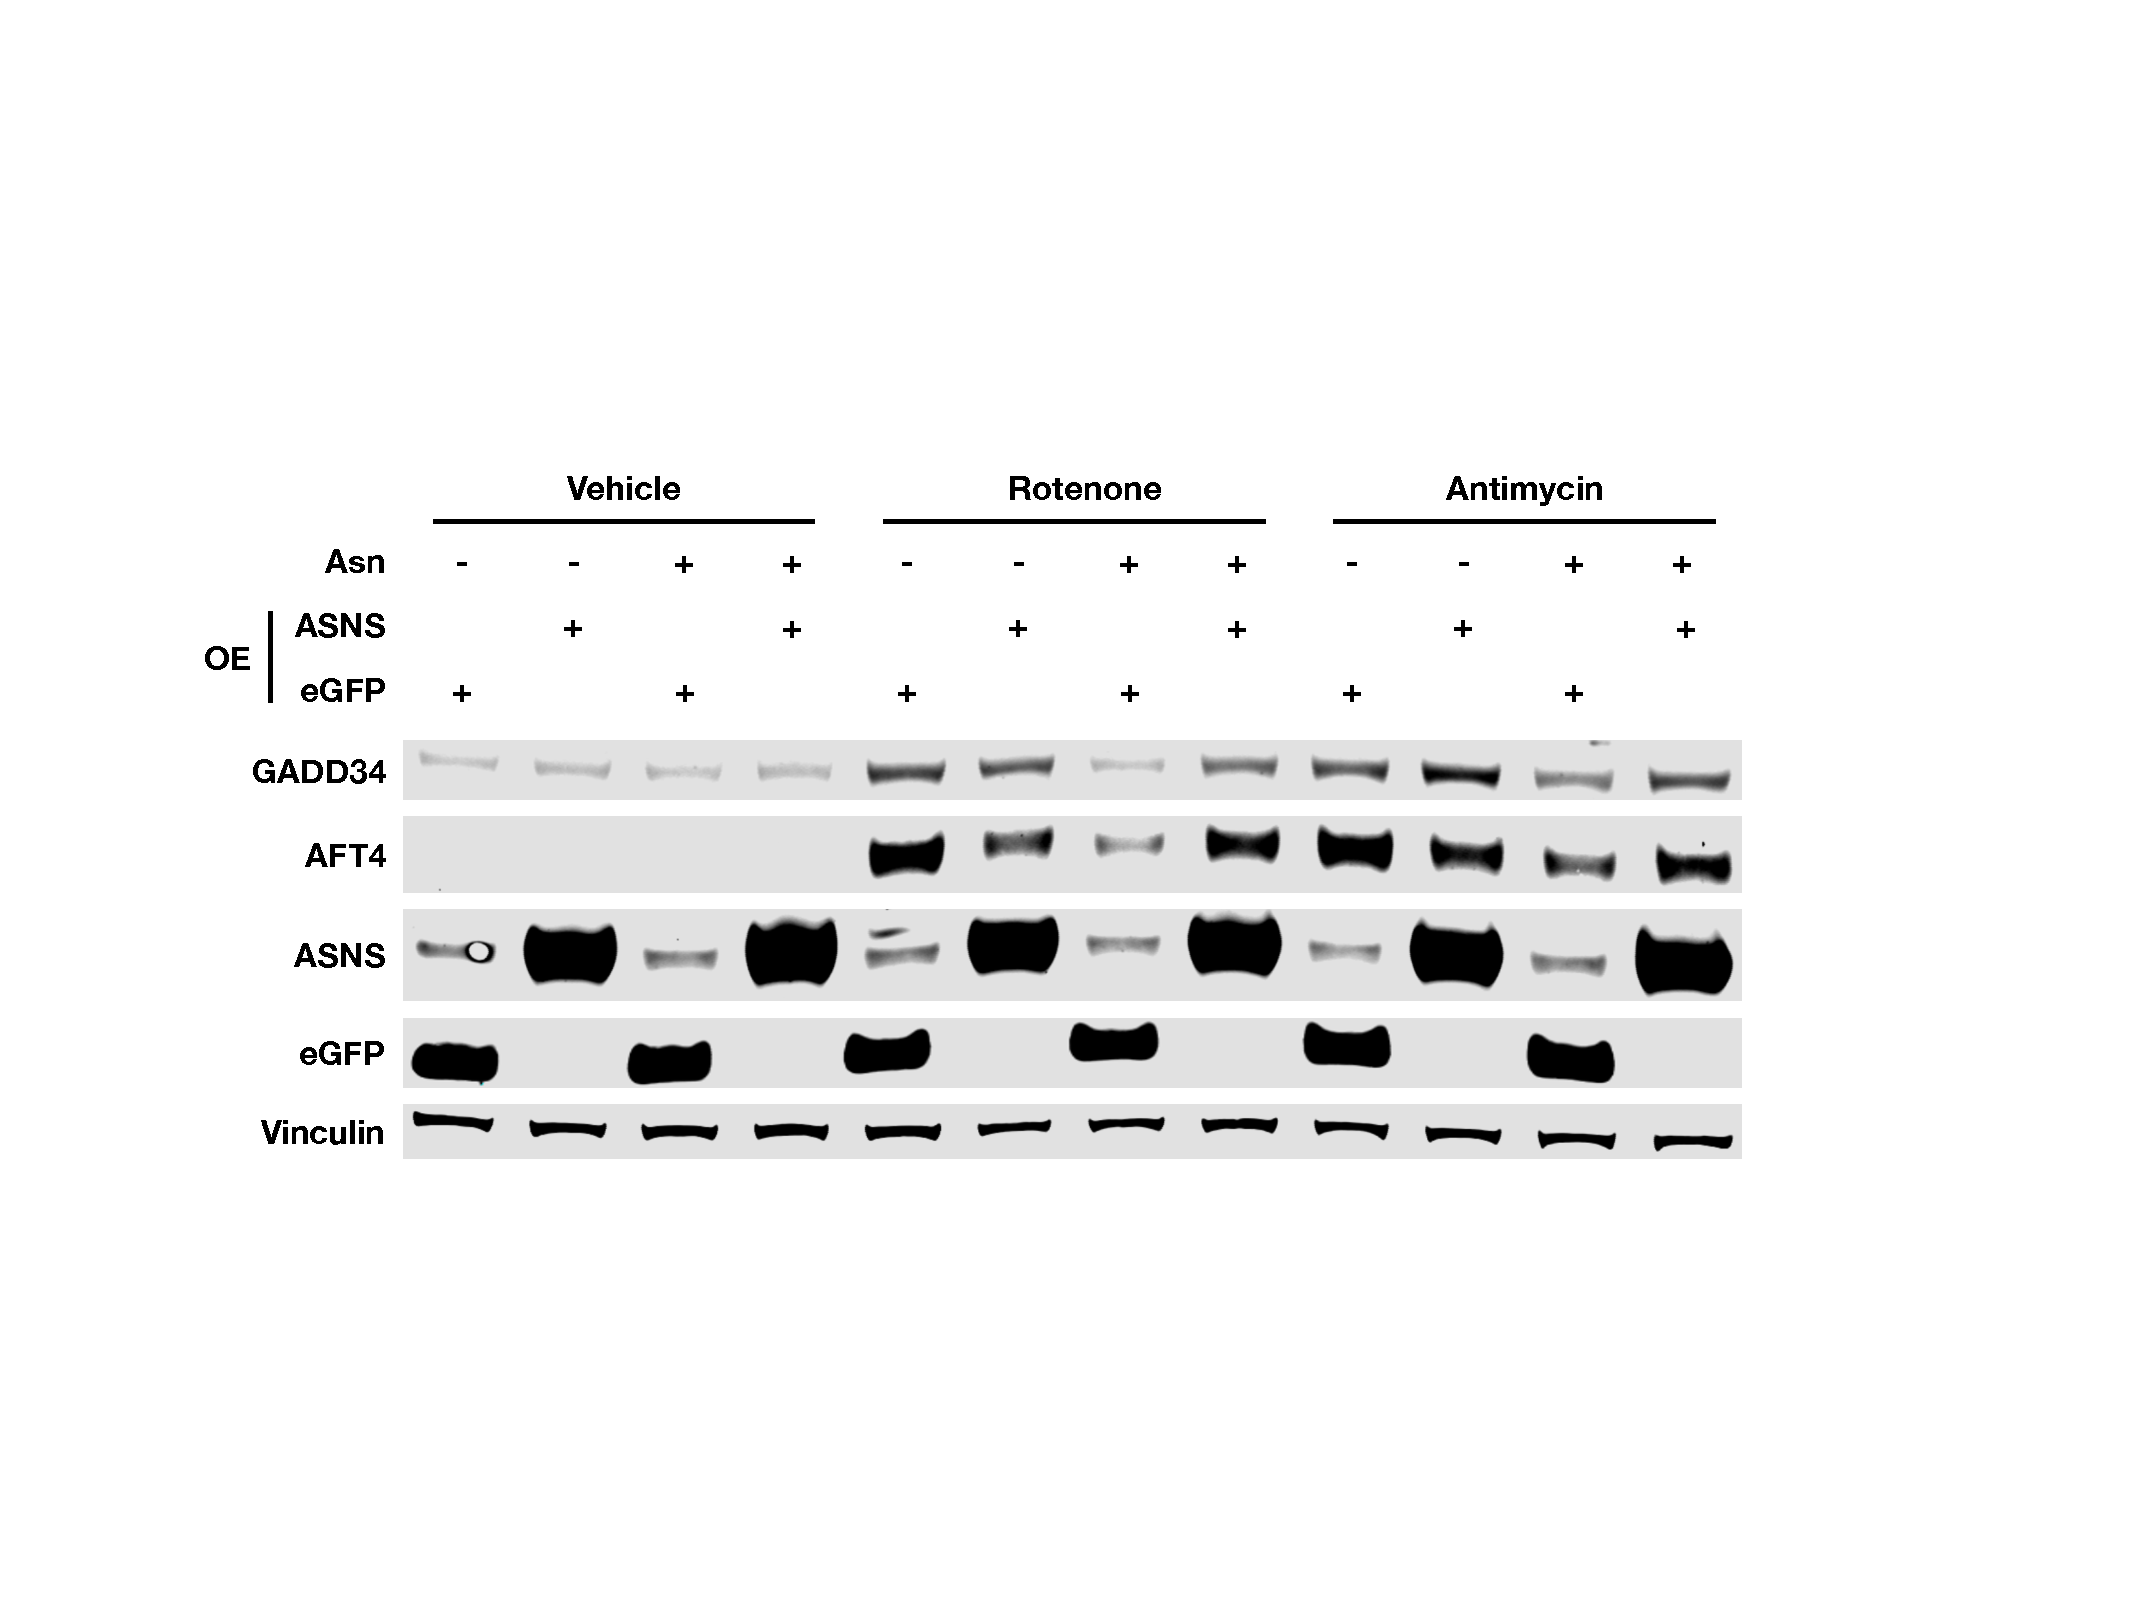
\includegraphics[width=\textwidth]{figures/sapp/ISR/HT1080_ISR_ASNS_OE.pdf}
         \caption{Western blot, eGFP/ASNS polyclonal}
         \label{fig:sapp:ISR:HT1080_ISR_ASNS_OE}
     \end{subfigure}
        \caption[ASNS OE, rotenone/antimycin induced ISR]{
        Effect of ASNS over-expression (eGFP control) on ATF4 reporter assay of ETC inhibitor induced ISR (parental HT1080 low baseline clone).
        For ATF4 reporter treatments was initiated by 10x spike-in, for western blot fresh media was added with drug at time zero.
        Using 100 nM rotenone and 1 µM antimycin.
        }
        \label{fig:sapp:ISR:ASNS_ISR}
\end{figure}






\FloatBarrier
\subsection{GCN2 relation to rotenone induced ISR in 293T}
Now, one would think that ETC inhibitor induced ISR is induced through Asp/Asn depletion and thus mediated by GCN2 and thus a GCN2 knockout should not upregulate ATF4.
We only have a confirmed GCN2 knockout in 293T cells and therefore tried with these.
Strangely, ISR in 293T cells was not reverted well with Asp/Asn, but even more strange the GCN2 KO cells did not have ablated ATF4.

\begin{figure}[ht]
    \centering
    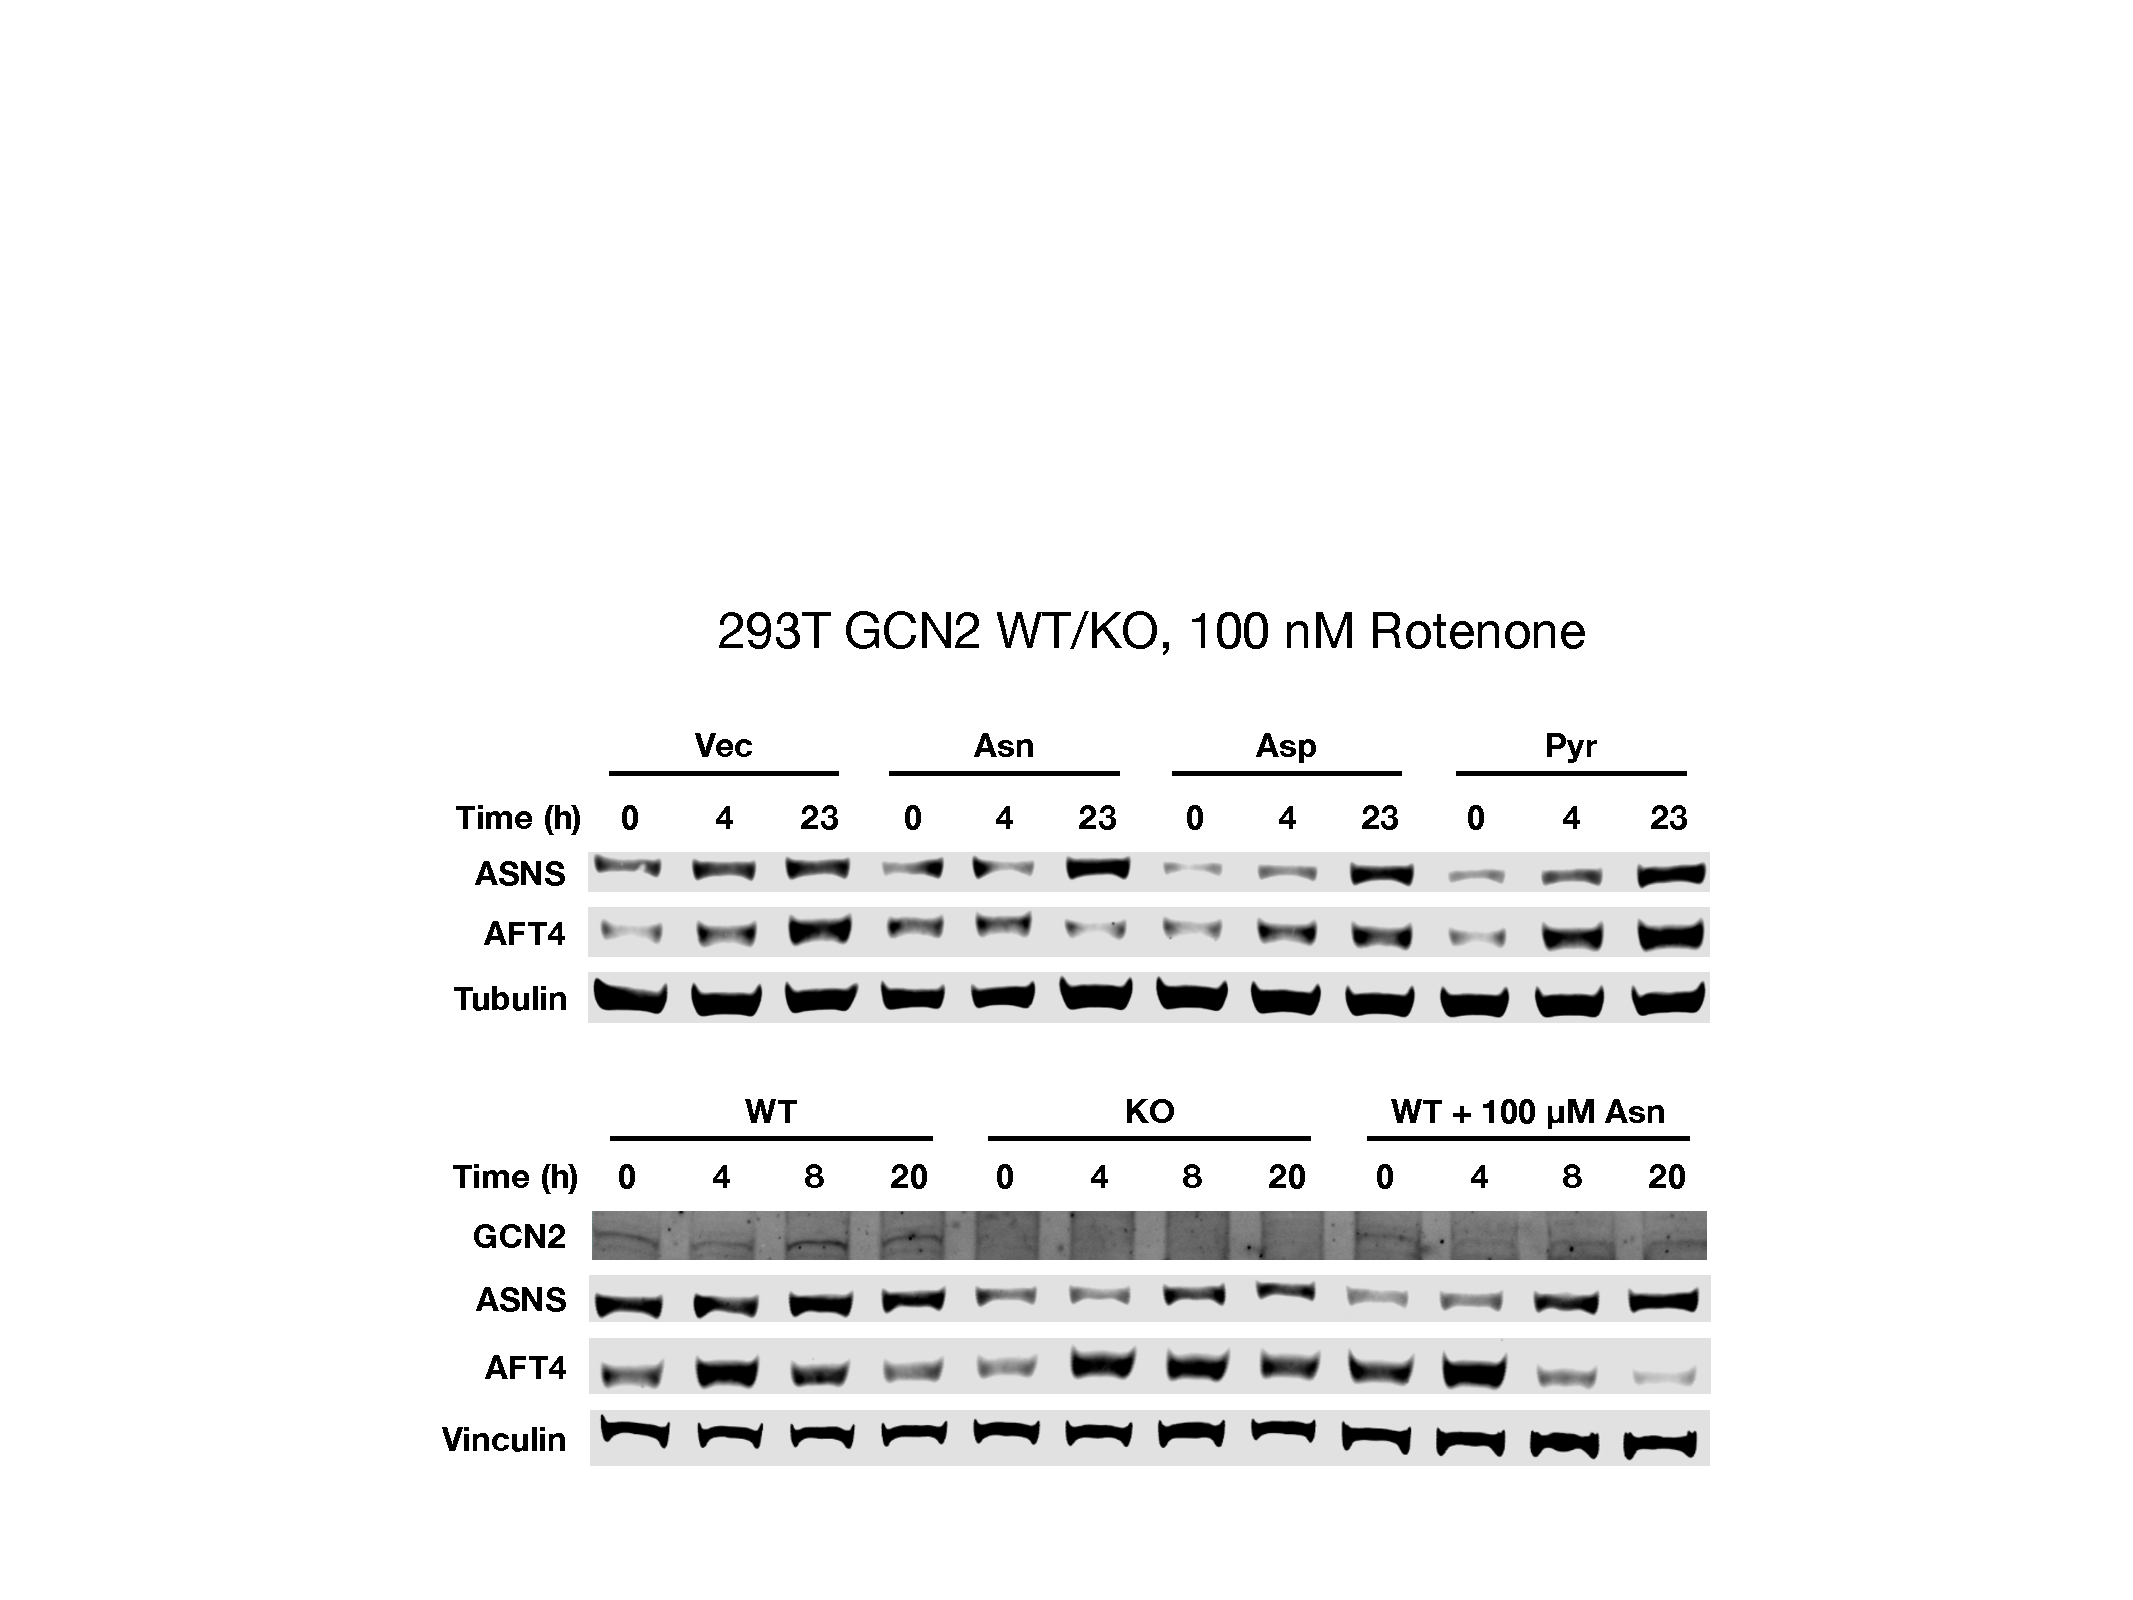
\includegraphics[width=0.70\textwidth]{figures/sapp/ISR/293T_GCN2_ISR.pdf}
    \caption[ATF4 post mito inhib. GCN2 KO, western]{
    Rotenone treatment was initiated by adding fresh media with 100 nM rotenone at time zero.
    Rescue conditions: Asn (500 µM), Asp (30 mM) or Pyr (2 mM) was also added to media >1 h before time zero.
    }
    \label{fig:sapp:ISR:293T_GCN2_ISR}
\end{figure}







\section{GOT DKO validation}





























